% Options for packages loaded elsewhere
\PassOptionsToPackage{unicode}{hyperref}
\PassOptionsToPackage{hyphens}{url}
%
\documentclass[
  11pt,
  letterpaper,
]{scrbook}

\usepackage{amsmath,amssymb}
\usepackage{iftex}
\ifPDFTeX
  \usepackage[T1]{fontenc}
  \usepackage[utf8]{inputenc}
  \usepackage{textcomp} % provide euro and other symbols
\else % if luatex or xetex
  \usepackage{unicode-math}
  \defaultfontfeatures{Scale=MatchLowercase}
  \defaultfontfeatures[\rmfamily]{Ligatures=TeX,Scale=1}
\fi
\usepackage{lmodern}
\ifPDFTeX\else  
    % xetex/luatex font selection
\fi
% Use upquote if available, for straight quotes in verbatim environments
\IfFileExists{upquote.sty}{\usepackage{upquote}}{}
\IfFileExists{microtype.sty}{% use microtype if available
  \usepackage[]{microtype}
  \UseMicrotypeSet[protrusion]{basicmath} % disable protrusion for tt fonts
}{}
\makeatletter
\@ifundefined{KOMAClassName}{% if non-KOMA class
  \IfFileExists{parskip.sty}{%
    \usepackage{parskip}
  }{% else
    \setlength{\parindent}{0pt}
    \setlength{\parskip}{6pt plus 2pt minus 1pt}}
}{% if KOMA class
  \KOMAoptions{parskip=half}}
\makeatother
\usepackage{xcolor}
\setlength{\emergencystretch}{3em} % prevent overfull lines
\setcounter{secnumdepth}{5}
% Make \paragraph and \subparagraph free-standing
\makeatletter
\ifx\paragraph\undefined\else
  \let\oldparagraph\paragraph
  \renewcommand{\paragraph}{
    \@ifstar
      \xxxParagraphStar
      \xxxParagraphNoStar
  }
  \newcommand{\xxxParagraphStar}[1]{\oldparagraph*{#1}\mbox{}}
  \newcommand{\xxxParagraphNoStar}[1]{\oldparagraph{#1}\mbox{}}
\fi
\ifx\subparagraph\undefined\else
  \let\oldsubparagraph\subparagraph
  \renewcommand{\subparagraph}{
    \@ifstar
      \xxxSubParagraphStar
      \xxxSubParagraphNoStar
  }
  \newcommand{\xxxSubParagraphStar}[1]{\oldsubparagraph*{#1}\mbox{}}
  \newcommand{\xxxSubParagraphNoStar}[1]{\oldsubparagraph{#1}\mbox{}}
\fi
\makeatother


\providecommand{\tightlist}{%
  \setlength{\itemsep}{0pt}\setlength{\parskip}{0pt}}\usepackage{longtable,booktabs,array}
\usepackage{calc} % for calculating minipage widths
% Correct order of tables after \paragraph or \subparagraph
\usepackage{etoolbox}
\makeatletter
\patchcmd\longtable{\par}{\if@noskipsec\mbox{}\fi\par}{}{}
\makeatother
% Allow footnotes in longtable head/foot
\IfFileExists{footnotehyper.sty}{\usepackage{footnotehyper}}{\usepackage{footnote}}
\makesavenoteenv{longtable}
\usepackage{graphicx}
\makeatletter
\def\maxwidth{\ifdim\Gin@nat@width>\linewidth\linewidth\else\Gin@nat@width\fi}
\def\maxheight{\ifdim\Gin@nat@height>\textheight\textheight\else\Gin@nat@height\fi}
\makeatother
% Scale images if necessary, so that they will not overflow the page
% margins by default, and it is still possible to overwrite the defaults
% using explicit options in \includegraphics[width, height, ...]{}
\setkeys{Gin}{width=\maxwidth,height=\maxheight,keepaspectratio}
% Set default figure placement to htbp
\makeatletter
\def\fps@figure{htbp}
\makeatother
% definitions for citeproc citations
\NewDocumentCommand\citeproctext{}{}
\NewDocumentCommand\citeproc{mm}{%
  \begingroup\def\citeproctext{#2}\cite{#1}\endgroup}
\makeatletter
 % allow citations to break across lines
 \let\@cite@ofmt\@firstofone
 % avoid brackets around text for \cite:
 \def\@biblabel#1{}
 \def\@cite#1#2{{#1\if@tempswa , #2\fi}}
\makeatother
\newlength{\cslhangindent}
\setlength{\cslhangindent}{1.5em}
\newlength{\csllabelwidth}
\setlength{\csllabelwidth}{3em}
\newenvironment{CSLReferences}[2] % #1 hanging-indent, #2 entry-spacing
 {\begin{list}{}{%
  \setlength{\itemindent}{0pt}
  \setlength{\leftmargin}{0pt}
  \setlength{\parsep}{0pt}
  % turn on hanging indent if param 1 is 1
  \ifodd #1
   \setlength{\leftmargin}{\cslhangindent}
   \setlength{\itemindent}{-1\cslhangindent}
  \fi
  % set entry spacing
  \setlength{\itemsep}{#2\baselineskip}}}
 {\end{list}}
\usepackage{calc}
\newcommand{\CSLBlock}[1]{\hfill\break\parbox[t]{\linewidth}{\strut\ignorespaces#1\strut}}
\newcommand{\CSLLeftMargin}[1]{\parbox[t]{\csllabelwidth}{\strut#1\strut}}
\newcommand{\CSLRightInline}[1]{\parbox[t]{\linewidth - \csllabelwidth}{\strut#1\strut}}
\newcommand{\CSLIndent}[1]{\hspace{\cslhangindent}#1}

% \usepackage{amsmath,amssymb,mathtools}
\usepackage{enumerate}
\usepackage{geometry}
\geometry{hmargin=1.2in}

\usepackage{booktabs}
\usepackage{amssymb}
\makeatletter
\def\thm@space@setup{%
  \thm@preskip=8pt plus 2pt minus 4pt
  \thm@postskip=\thm@preskip
}
\makeatother

\usepackage{framed,color}
\definecolor{shadecolor}{RGB}{248,248,248}

\renewcommand{\textfraction}{0.05}
\renewcommand{\topfraction}{0.8}
\renewcommand{\bottomfraction}{0.8}
\renewcommand{\floatpagefraction}{0.75}

%\let\oldhref\href
%\renewcommand{\href}[2]{#2\footnote{\url{#1}}}

\ifxetex
  \usepackage{letltxmacro}
  \setlength{\XeTeXLinkMargin}{1pt}
  \LetLtxMacro\SavedIncludeGraphics\includegraphics
  \def\includegraphics#1#{% #1 catches optional stuff (star/opt. arg.)
    \IncludeGraphicsAux{#1}%
  }%
  \newcommand*{\IncludeGraphicsAux}[2]{%
    \XeTeXLinkBox{%
      \SavedIncludeGraphics#1{#2}%
    }%
  }%
\fi

\makeatletter
\newenvironment{kframe}{%
\medskip{}
\setlength{\fboxsep}{.8em}
 \def\at@end@of@kframe{}%
 \ifinner\ifhmode%
  \def\at@end@of@kframe{\end{minipage}}%
  \begin{minipage}{\columnwidth}%
 \fi\fi%
 \def\FrameCommand##1{\hskip\@totalleftmargin \hskip-\fboxsep
 \colorbox{shadecolor}{##1}\hskip-\fboxsep
     % There is no \\@totalrightmargin, so:
     \hskip-\linewidth \hskip-\@totalleftmargin \hskip\columnwidth}%
 \MakeFramed {\advance\hsize-\width
   \@totalleftmargin\z@ \linewidth\hsize
   \@setminipage}}%
 {\par\unskip\endMakeFramed%
 \at@end@of@kframe}
\makeatother

\makeatletter
\@ifundefined{Shaded}{
}{\renewenvironment{Shaded}{\begin{kframe}}{\end{kframe}}}
\makeatother

\newenvironment{rmdblock}[1]
  {
  \begin{itemize}
  \renewcommand{\labelitemi}{
    \raisebox{-.7\height}[0pt][0pt]{
      {\setkeys{Gin}{width=3em,keepaspectratio}\includegraphics{images/#1}}
    }
  }
  \setlength{\fboxsep}{1em}
  \begin{kframe}
  \item
  }
  {
  \end{kframe}
  \end{itemize}
  }
\newenvironment{rmdnote}
  {\begin{rmdblock}{note}}
  {\end{rmdblock}}
\newenvironment{rmdcaution}
  {\begin{rmdblock}{caution}}
  {\end{rmdblock}}
\newenvironment{rmdimportant}
  {\begin{rmdblock}{important}}
  {\end{rmdblock}}
\newenvironment{rmdtip}
  {\begin{rmdblock}{tip}}
  {\end{rmdblock}}
\newenvironment{rmdwarning}
  {\begin{rmdblock}{warning}}
  {\end{rmdblock}}
\usepackage{mathrsfs}
\DeclareMathAlphabet{\mathcrl}{U}{rsfs}{m}{n}
\usepackage{utopia}
\DeclareMathAlphabet{\mathcal}{OMS}{cmsy}{m}{n}
\usepackage{pdfpages}
\usepackage{booktabs}
\usepackage{longtable}
\usepackage{array}
\usepackage{multirow}
\usepackage{wrapfig}
\usepackage{float}
\usepackage{colortbl}
\usepackage{pdflscape}
\usepackage{tabu}
\usepackage{threeparttable}
\usepackage{threeparttablex}
\usepackage[normalem]{ulem}
\usepackage{makecell}
\usepackage{xcolor}
\makeatletter
\@ifpackageloaded{tcolorbox}{}{\usepackage[skins,breakable]{tcolorbox}}
\@ifpackageloaded{fontawesome5}{}{\usepackage{fontawesome5}}
\definecolor{quarto-callout-color}{HTML}{909090}
\definecolor{quarto-callout-note-color}{HTML}{0758E5}
\definecolor{quarto-callout-important-color}{HTML}{CC1914}
\definecolor{quarto-callout-warning-color}{HTML}{EB9113}
\definecolor{quarto-callout-tip-color}{HTML}{00A047}
\definecolor{quarto-callout-caution-color}{HTML}{FC5300}
\definecolor{quarto-callout-color-frame}{HTML}{acacac}
\definecolor{quarto-callout-note-color-frame}{HTML}{4582ec}
\definecolor{quarto-callout-important-color-frame}{HTML}{d9534f}
\definecolor{quarto-callout-warning-color-frame}{HTML}{f0ad4e}
\definecolor{quarto-callout-tip-color-frame}{HTML}{02b875}
\definecolor{quarto-callout-caution-color-frame}{HTML}{fd7e14}
\makeatother
\makeatletter
\@ifpackageloaded{bookmark}{}{\usepackage{bookmark}}
\makeatother
\makeatletter
\@ifpackageloaded{caption}{}{\usepackage{caption}}
\AtBeginDocument{%
\ifdefined\contentsname
  \renewcommand*\contentsname{Table of contents}
\else
  \newcommand\contentsname{Table of contents}
\fi
\ifdefined\listfigurename
  \renewcommand*\listfigurename{List of Figures}
\else
  \newcommand\listfigurename{List of Figures}
\fi
\ifdefined\listtablename
  \renewcommand*\listtablename{List of Tables}
\else
  \newcommand\listtablename{List of Tables}
\fi
\ifdefined\figurename
  \renewcommand*\figurename{Figure}
\else
  \newcommand\figurename{Figure}
\fi
\ifdefined\tablename
  \renewcommand*\tablename{Table}
\else
  \newcommand\tablename{Table}
\fi
}
\@ifpackageloaded{float}{}{\usepackage{float}}
\floatstyle{ruled}
\@ifundefined{c@chapter}{\newfloat{codelisting}{h}{lop}}{\newfloat{codelisting}{h}{lop}[chapter]}
\floatname{codelisting}{Listing}
\newcommand*\listoflistings{\listof{codelisting}{List of Listings}}
\usepackage{amsthm}
\theoremstyle{definition}
\newtheorem{definition}{Definition}[chapter]
\theoremstyle{definition}
\newtheorem{example}{Example}[chapter]
\theoremstyle{remark}
\AtBeginDocument{\renewcommand*{\proofname}{Proof}}
\newtheorem*{remark}{Remark}
\newtheorem*{solution}{Solution}
\newtheorem{refremark}{Remark}[chapter]
\newtheorem{refsolution}{Solution}[chapter]
\makeatother
\makeatletter
\makeatother
\makeatletter
\@ifpackageloaded{caption}{}{\usepackage{caption}}
\@ifpackageloaded{subcaption}{}{\usepackage{subcaption}}
\makeatother

\ifLuaTeX
\usepackage[bidi=basic]{babel}
\else
\usepackage[bidi=default]{babel}
\fi
\babelprovide[main,import]{english}
% get rid of language-specific shorthands (see #6817):
\let\LanguageShortHands\languageshorthands
\def\languageshorthands#1{}
\ifLuaTeX
  \usepackage{selnolig}  % disable illegal ligatures
\fi
\usepackage{bookmark}

\IfFileExists{xurl.sty}{\usepackage{xurl}}{} % add URL line breaks if available
\urlstyle{same} % disable monospaced font for URLs
\hypersetup{
  pdftitle={MATH 60604A - Statistical Modelling},
  pdfauthor={Léo Belzile},
  pdflang={en},
  hidelinks,
  pdfcreator={LaTeX via pandoc}}


\title{MATH 60604A - Statistical Modelling}
\author{Léo Belzile}
\date{2024-08-26}

\begin{document}

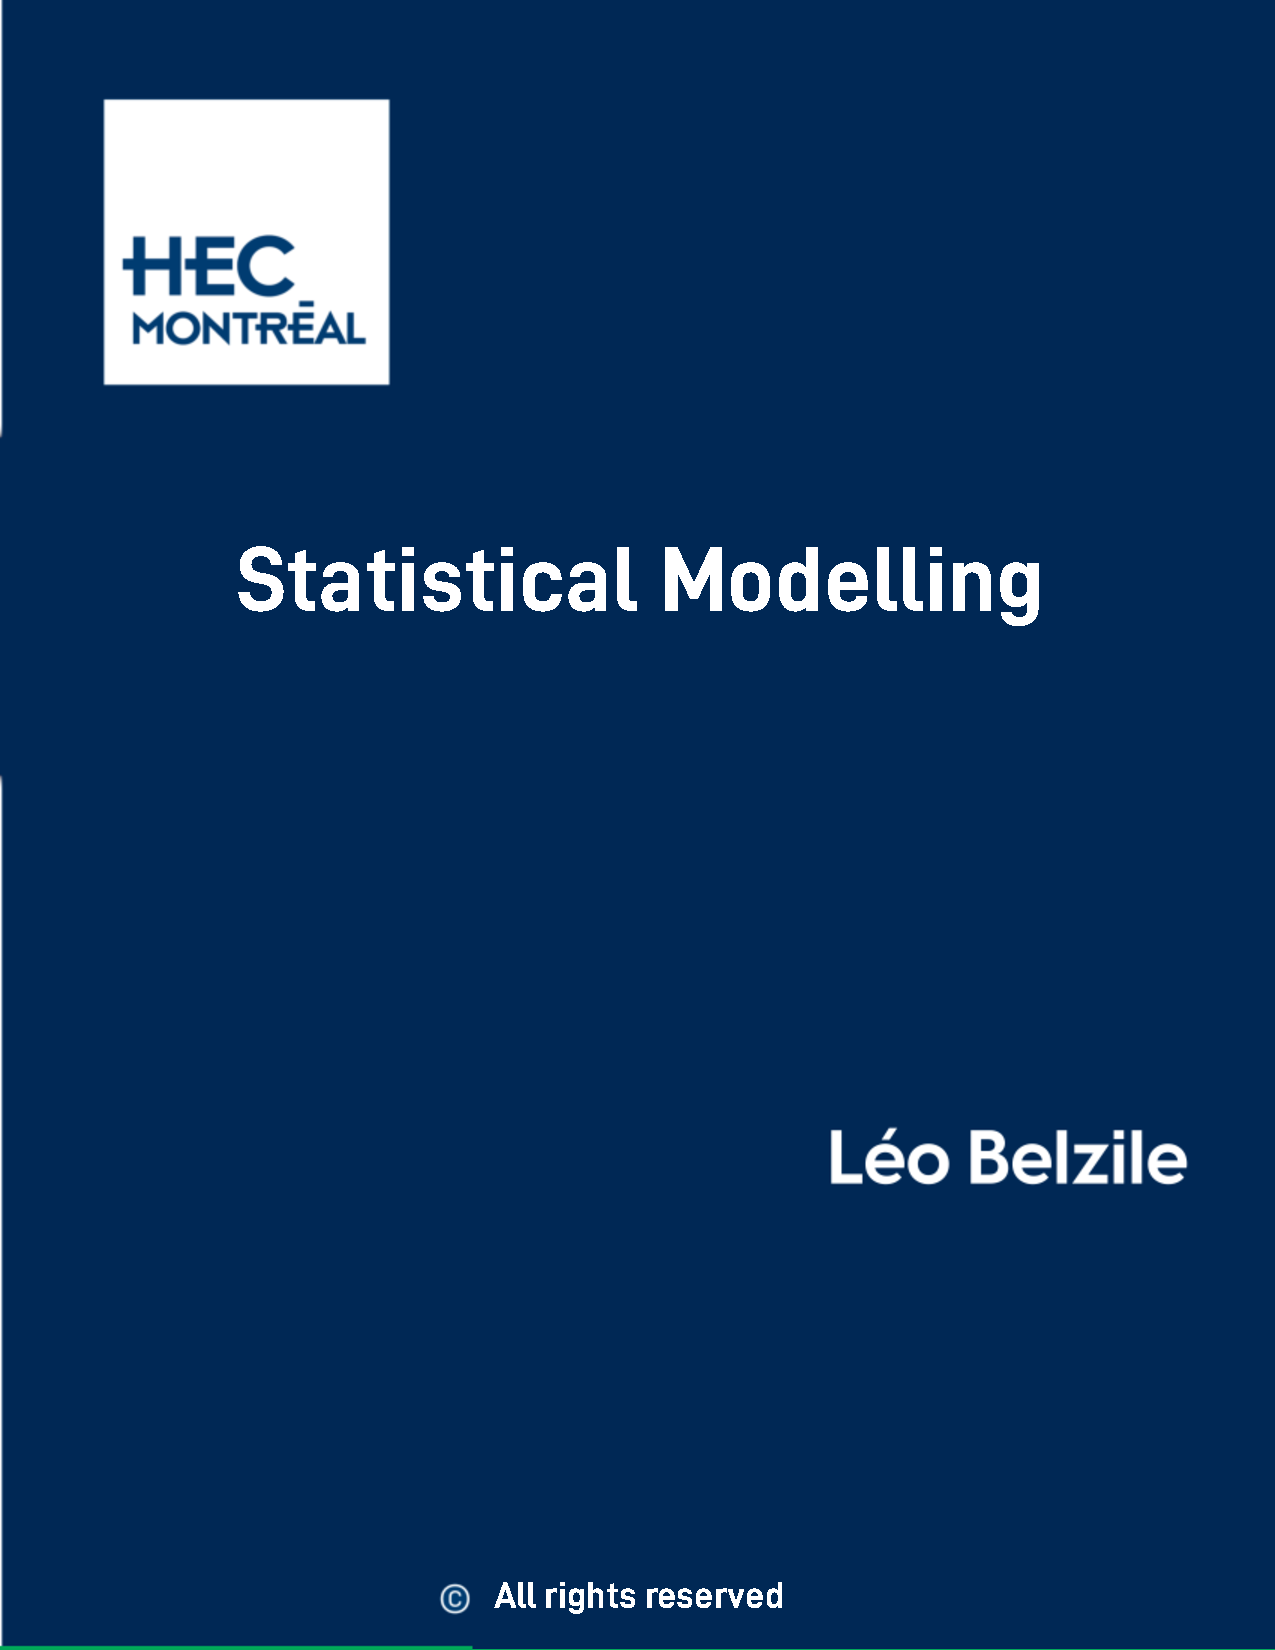
\includepdf{images/coverpage.pdf}

\renewcommand*\contentsname{Table of contents}
{
\setcounter{tocdepth}{2}
\tableofcontents
}

\mainmatter
\bookmarksetup{startatroot}

\chapter*{Welcome}\label{welcome}
\addcontentsline{toc}{chapter}{Welcome}

\markboth{Welcome}{Welcome}

These notes by Léo Belzile (HEC Montréal) are licensed under a
\href{http://creativecommons.org/licenses/by-nc-sa/4.0/}{Creative
Commons Attribution-NonCommercial-ShareAlike 4.0 International License}.

This course is about statistical modelling.

A famous quote attributed to George Box claims that

\begin{quote}
All models are wrong, but some are useful.
\end{quote}

This standpoint is reductive: Peter McCullagh and John Nelder wrote in
the preamble of their book (emphasis mine)

\begin{quote}
Modelling in science remains, partly at least, an art. Some principles
do exist, however, to guide the modeller. The first is that all models
are wrong; \textbf{some, though, are better} than others and we can
\textbf{search for the better ones}. At the same time we must recognize
that eternal truth is not within our grasp.
\end{quote}

And this quote by David R. Cox adds to the point:

\begin{quote}
\ldots it does not seem helpful just to say that all models are wrong.
The very word model implies simplification and idealization. The idea
that complex physical, biological or sociological systems can be exactly
described by a few formulae is patently absurd. The construction of
idealized representations that \textbf{capture important stable aspects
of such systems} is, however, a vital part of general scientific
analysis and statistical models, especially substantive ones, do not
seem essentially different from other kinds of model.
\end{quote}

Why use models?
\href{https://krugman.blogs.nytimes.com/2010/11/18/debt-deleveraging-and-the-liquidity-trap/}{Paul
Krugman wrote in 2010 in his blog}

\begin{quote}
The answer I'd give is that models are an enormously important tool for
clarifying your thought. You don't have to literally believe your model
--- in fact, you're a fool if you do --- to believe that putting
together a simplified but complete account of how things work, with all
the eyes crossed and teas dotted or something, helps you gain a much
more sophisticated understanding of the real situation. People who don't
use models end up relying on slogans that are much more simplistic than
the models
\end{quote}

\section*{Course content}\label{course-content}
\addcontentsline{toc}{section}{Course content}

\markright{Course content}

There are two main data type: \textbf{experimental} data are typically
collected in a control environment following a research protocol with a
particular experimental design: they serve to answer questions specified
ahead of time. This approach is highly desirable to avoid the garden of
forking paths
\href{http://www.stat.columbia.edu/~gelman/research/unpublished/p_hacking.pdf}{(researchers
unfortunately tend to refine or change their hypothesis in light of
data, which invalidates their findings} --- preregistration alleviates
this somewhat). While experimental data are highly desirable, it is not
always possible to collect experimental data: for example, an economist
cannot modify interest rates to see how it impacts consumer savings.
When data have been collected beforehand without intervention (for other
purposes), these are called \textbf{observational}. These will be the
ones most frequently encountered.

A stochastic model will comprise two ingredients: a distribution for the
random data and a formula linking the parameters or the conditional
expectation of a response variable \(Y\) to a set of explanatories
\(\mathbf{X}\). A model can serve to either predict new outcomes
(predictive modelling) or else to test research hypothesis about the
effect of the explanatory variables on the response (explanatory model).
These two objectives are of course not mutually exclusive even if we
distinguish in practice inference and prediction.

A predictive model gives predictions of \(Y\) for different combinations
of explanatory variables or future data. For example, one could try to
forecast the enery consumption of a house as a function of weather, the
number of inhabitants and its size. Black boxes used in machine learning
are often used solely for prediction: these models are not easily
interpreted and they often ignore the data structure.

By constrast, explicative models are often simple and interpretable:
regression models are often used for inference purpose and we will focus
on these. The following examples will be covered in class or as part of
the exercices:

\begin{itemize}
\tightlist
\item
  Are sequential decisions in online shop (buying or not, then selecting
  the quantity) preferable to integrated decisions
  (\citeproc{ref-Duke.Amir:2023}{Duke and Amir 2023})?
\item
  Determining what is the most distracting for road users: talking on a
  cellphone, texting or checking your smartwatch
  (\citeproc{ref-Brodeur:2021}{Brodeur et al. 2021})?
\item
  What is the impact of inconsistencies between product description and
  the displayed image (\citeproc{ref-Lee.Choi:2019}{Lee and Choi 2019})?
\item
  Is the price of gasoline more expensive in the Gaspé peninsula than in
  the rest of Quebec?
  \href{https://ici.radio-canada.ca/nouvelle/1463520/prix-essence-gaspesie-rapport-regie-energie}{A
  report of the \emph{Régie de l'énergie} examines the question}
\item
  Are driving tests in the UK easier if you live in a rural area?
  \href{https://www.theguardian.com/world/2019/aug/23/an-easy-ride-scottish-village-fuels-debate-driving-test-pass-rates}{An
  analysis of \emph{The Guardian}} hints that it is the case.
\item
  What is the environmental perception of a package that includes
  cardboard over a plastic container
  (\citeproc{ref-Sokolova:2023}{Sokolova, Krishna, and Döring 2023})?
\item
  What is the psychological impact of suggested amounts on donations
  (\citeproc{ref-Moon.VanEpps:2023}{Moon and VanEpps 2023})?
\item
  What are the benefits of face-to-face meetings, rather than via
  videoconference tools? Brucks and Levav
  (\citeproc{ref-Brucks.Levav:2022}{2022}) suggests a decrease in the
  number of creative ideas and interactions when meeting online.
\end{itemize}

\bookmarksetup{startatroot}

\chapter{Introduction}\label{intro}

This chapter reviews some basic notions of probability and statistics
that are normally covered in undergraduate or college.

\section{Population and samples}\label{population-sample}

Statistics is the science of uncertainty quantification: of paramount
importance is the notion of randomness. Generally, we will seek to
estimate characteristics of a population using only a sample (a
sub-group of the population of smaller size).

The \textbf{population of interest} is a collection of individuals which
the study targets. For example, the Labour Force Survey (LFS) is a
monthly study conducted by Statistics Canada, who define the target
population as ``all members of the selected household who are 15 years
old and older, whether they work or not.'' Asking every Canadian meeting
this definition would be costly and the process would be long: the
characteristic of interest (employment) is also a snapshot in time and
can vary when the person leaves a job, enters the job market or become
unemployed.

In general, we therefore consider only \textbf{samples} to gather the
information we seek to obtain. The purpose of \textbf{statistical
inference} is to draw conclusions about the population, but using only a
share of the latter and accounting for sources of variability. George
Gallup made this great analogy between sample and population:

\begin{quote}
One spoonful can reflect the taste of the whole pot, if the soup is
well-stirred
\end{quote}

A \textbf{sample} is a random sub-group of individuals drawn from the
population. Creation of sampling plans is a complex subject and
semester-long sampling courses would be required to evens scratch the
surface of the topic. Even if we won't be collecting data, keep in mind
the following information: for a sample to be good, it must be
representative of the population under study. Selection bias must be
avoided, notably samples of friends or of people sharing opinions.

Because the individuals are selected at \textbf{random} to be part of
the sample, the measurement of the characteristic of interest will also
be random and change from one sample to the next. However, larger
samples of the same quality carry more information and our estimator
will be more precise. Sample size is not guarantee of quality, as the
following example demonstrates.

\begin{example}[Polling for the 1936 USA Presidential
Election]\protect\hypertarget{exm-Galluppoll}{}\label{exm-Galluppoll}

\emph{The Literary Digest} surveyed 10 millions people by mail to know
voting preferences for the 1936 USA Presidential Election. A sizeable
share, 2.4 millions answered, giving Alf Landon (57\%) over incumbent
President Franklin D. Roosevelt (43\%). The latter nevertheless won in a
landslide election with 62\% of votes cast, a 19\% forecast error.
\href{https://www.jstor.org/stable/2749114}{Biased sampling and
differential non-response are mostly responsible for the error:} the
sampling frame was built using ``phone number directories, drivers'
registrations, club memberships, etc.'', all of which skewed the sample
towards rich upper class white people more susceptible to vote for the
GOP.

In contrast, Gallup correctly predicted the outcome by polling (only)
50K inhabitants.
\href{https://ozanozbey.medium.com/two-lessons-of-sampling-bias-from-1936-us-election-e4e96bd42be}{Read
the full story here.}

\end{example}

\subsection{Variable type}\label{variable-type}

\begin{itemize}
\tightlist
\item
  a \textbf{variable} represents a characteristic of the population, for
  example the sex of an individual, the price of an item, etc.
\item
  an \textbf{observation} is a set of measures (variables) collected
  under identical conditions for an individual or at a given time.
\end{itemize}

\begin{longtable}[]{@{}
  >{\raggedleft\arraybackslash}p{(\columnwidth - 12\tabcolsep) * \real{0.0923}}
  >{\raggedright\arraybackslash}p{(\columnwidth - 12\tabcolsep) * \real{0.1231}}
  >{\raggedright\arraybackslash}p{(\columnwidth - 12\tabcolsep) * \real{0.1692}}
  >{\raggedright\arraybackslash}p{(\columnwidth - 12\tabcolsep) * \real{0.1385}}
  >{\raggedright\arraybackslash}p{(\columnwidth - 12\tabcolsep) * \real{0.2615}}
  >{\raggedleft\arraybackslash}p{(\columnwidth - 12\tabcolsep) * \real{0.1385}}
  >{\raggedright\arraybackslash}p{(\columnwidth - 12\tabcolsep) * \real{0.0769}}@{}}

\caption{\label{tbl-data-renfe}First lines of the \texttt{renfe}
database, which contains the price of 10K train tickets between Madrid
and Barcelona. The columns \texttt{price} and \texttt{duration}
represent continuous variables, all others are categorical.}

\tabularnewline

\toprule\noalign{}
\begin{minipage}[b]{\linewidth}\raggedleft
price
\end{minipage} & \begin{minipage}[b]{\linewidth}\raggedright
type
\end{minipage} & \begin{minipage}[b]{\linewidth}\raggedright
class
\end{minipage} & \begin{minipage}[b]{\linewidth}\raggedright
fare
\end{minipage} & \begin{minipage}[b]{\linewidth}\raggedright
dest
\end{minipage} & \begin{minipage}[b]{\linewidth}\raggedleft
duration
\end{minipage} & \begin{minipage}[b]{\linewidth}\raggedright
wday
\end{minipage} \\
\midrule\noalign{}
\endhead
\bottomrule\noalign{}
\endlastfoot
143.4 & AVE & Preferente & Promo & Barcelona-Madrid & 190 & 6 \\
181.5 & AVE & Preferente & Flexible & Barcelona-Madrid & 190 & 2 \\
86.8 & AVE & Preferente & Promo & Barcelona-Madrid & 165 & 7 \\
86.8 & AVE & Preferente & Promo & Barcelona-Madrid & 190 & 7 \\
69.0 & AVE-TGV & Preferente & Promo & Barcelona-Madrid & 175 & 4 \\

\end{longtable}

The choice of statistical model and test depends on the underlying type
of the data collected. There are many choices: quantitative (discrete or
continuous) if the variables are numeric, or qualitative (binary,
nominal, ordinal) if they can be described using an adjective; I prefer
the term categorical, which is more evocative.

Most of the models we will deal with are so-called regression models, in
which the mean of a quantitative variable is a function of other
variables, termed explanatories. There are two types of numerical
variables

\begin{itemize}
\tightlist
\item
  a discrete variable takes a finite or countable number of values,
  prime examples being binary variables or count variables.
\item
  a continuous variable can take (in theory) an infinite possible number
  of values, even when measurements are rounded or measured with a
  limited precision (time, width, mass). In many case, we could also
  consider discrete variables as continuous if they take enough values
  (e.g., money).
\end{itemize}

Categorical variables take only a finite of values. They are regrouped
in two groups,

\begin{itemize}
\tightlist
\item
  nominal if there is no ordering between levels (sex, color, country of
  origin) or
\item
  ordinal if they are ordered (Likert scale, salary scale) and this
  ordering should be reflected in graphs or tables.
\end{itemize}

We will bundle every categorical variable using arbitrary encoding for
the levels: for modelling, these variables taking \(K\) possible values
(or levels) must be transformed into a set of \(K-1\) binary 0/1
variables, the omitted level corresponding to a baseline. Failing to
declare categorical variables in your favorite software is a common
mistake, especially when these are saved in the database using integers
rather than strings.

\section{Random variable}\label{random-variable}

Suppose we wish to describe the behaviour of a stochastic phenomenon. To
this effect, one should enumerate the set of possible values taken by
the variable of interest and their probability: this is what is encoded
in the distribution.

Random variables are denoted using capital letters: for example
\(Y \sim \mathsf{normal}(\mu, \sigma^2)\) indicates that \(Y\) follows a
normal distribution with parameters \(\mu\) and \(\sigma>0.\) If the
values of the latter are left unspecified, we talk about the family of
distributions. When the values are given, for example \(\mu=0\) and
\(\sigma=1\), we deal with a single distribution for which a function
encode the probability of the underlying variable.

\begin{definition}[Distribution function, mass function and
density]\protect\hypertarget{def-cdf}{}\label{def-cdf}

The (cumulative) distribution function \(F(y)\) gives the cumulative
probability that an event doesn't exceed a given numerical value \(y\),
\(F(y) = \mathsf{Pr}(Y \leq y).\)

If \(Y\) is discrete, then it has atoms of non-zero probability and we
call \(f\) the mass function, and \(f(y)=\mathsf{Pr}(Y=y)\) gives the
probability of each outcome \(y.\) In the continuous case, no numerical
value has non-zero probability and so we consider intervals instead. The
density function \(f(x)\) is non-negative and satisfies
\(\int_{\mathbb{R}} f(x) \mathrm{d}x=1\): the integral over a set \(B\)
(the area under the curve) gives the probability of \(Y\) falling inside
\(B \in \mathbb{R}.\) It follows that the distribution function of a
continuous random variable is simply
\(F(y) = \int_{-\infty}^y f(x) \mathrm{d} x.\)

\begin{figure}[ht!]

{\centering 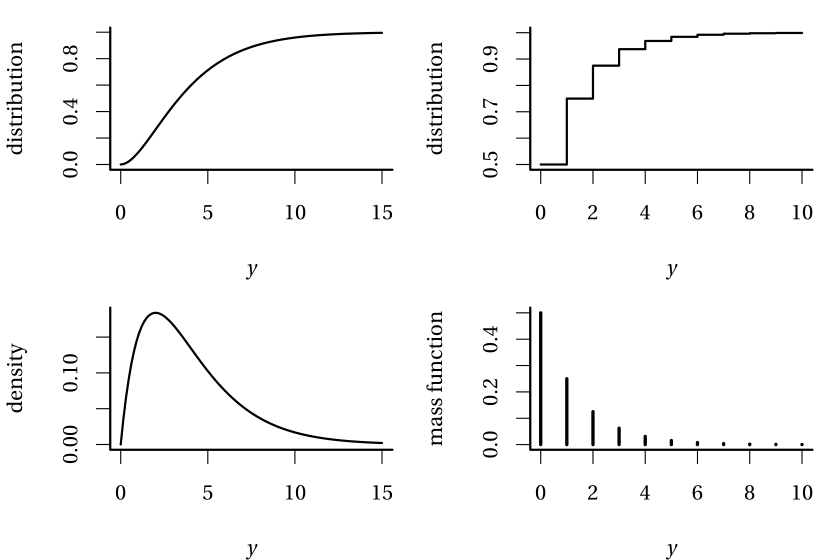
\includegraphics[width=0.85\textwidth,height=\textheight]{images/02-ttest-DF_illustration.png}

}

\caption{(Cumulative) distribution functions (top) and density/mass
functions (bottom) of continuous (left) and discrete (right) random
variables.}

\end{figure}%

\end{definition}

One of the first topics covered in introductory statistics is
descriptive statistics such as the mean and standard deviation. These
are estimators of (centered) moments, which characterise a random
variable. In the case of the standard normal distribution, the
expectation and variance fully characterize the distribution.

\begin{definition}[Moments]\protect\hypertarget{def-moments}{}\label{def-moments}

Let \(Y\) be a random variable with density (or mass) function \(f(x).\)
The \textbf{expectation} (or theoretical mean) of a continuous random
variable \(Y\) is \begin{align*}
\mathsf{E}(Y)=\int_{\mathbb{R}} x f(x) \mathrm{d} x.
\end{align*} In the discrete case, we set rather
\(\mu = \mathsf{E}(Y)=\sum_{x \in \mathcal{X}} x \mathsf{Pr}(X=x)\),
where \(\mathcal{X}\) denotes the support of \(Y\), the set of numerical
values at which the probability of \(Y\) is non-zero. More generally, we
can look at the expectation of a function \(g(x)\) for \(Y\), which is
nothing but the integral (or sum in the discrete case) of \(g(x)\)
weighted by the density or mass function of \(f(x).\) In the same
fashion, provided the integral is finite, the variance is \begin{align*}
\mathsf{Va}(Y)=\mathsf{E}\{Y-\mathsf{E}(Y)\}^2 \equiv \int_{\mathbb{R}} (x-\mu)^2 f(x) \mathrm{d} x.
\end{align*} The \textbf{standard deviation} is the square root of the
variance, \(\mathsf{sd}(Y)=\sqrt{\mathsf{Va}(Y)}\): it units are the
same as those of \(Y\) and are thus more easily interpreted.

The notion of moments can be extended to higher dimensions. Consider an
\(n\)-vector \(\boldsymbol{Y}.\) In the regression setting, the response
\(\boldsymbol{Y}\) would usually comprise repeated measures on an
individual, or even observations from a group of individuals.

The expected value (theoretical mean) of the vector \(\boldsymbol{Y}\)
is calculated componentwise, i.e., \begin{align*}
\mathsf{E}(\boldsymbol{Y}) &= \boldsymbol{\mu}=
\begin{pmatrix}
\mathsf{E}(Y_1) &
\cdots  &
\mathsf{E}(Y_n)
\end{pmatrix}^\top
\end{align*} whereas the second moment of \(\boldsymbol{Y}\) is encoded
in the \(n \times n\) \textbf{covariance} matrix \begin{align*}
\mathsf{Va}(\boldsymbol{Y}) &= \boldsymbol{\Sigma} = \begin{pmatrix} \mathsf{Va}(Y_1) & \mathsf{Co}(Y_1, Y_2)  & \cdots & \mathsf{Co}(Y_1, Y_n) \\
\mathsf{Co}(Y_2, Y_1) & \mathsf{Va}(Y_2) & \ddots & \vdots \\
\vdots & \ddots & \ddots & \vdots \\
\mathsf{Co}(Y_n, Y_1) & \mathsf{Co}(Y_n, Y_2) &\cdots & \mathsf{Va}(Y_n)
\end{pmatrix}
\end{align*} The \(i\)th diagonal element of \(\boldsymbol{\Sigma}\),
\(\sigma_{ii}=\sigma_i^2\), is the variance of \(Y_i\), whereas the
off-diagonal entries \(\sigma_{ij}=\sigma_{ji}\) \((i \neq j)\) are the
covariance of pairwise entries, with \begin{align*}
\mathsf{Co}(Y_i, Y_j) = \int_{\mathbb{R}^2} (y_i-\mu_i)(y_j-\mu_j) f_{Y_i, Y_j}(y_i, y_j) \mathrm{d} y_i \mathrm{d} y_j.
\end{align*} The covariance matrix \(\boldsymbol{\Sigma}\) is thus
symmetric. It is customary to normalize the pairwise dependence so they
do not depend on the component variance. The linear \textbf{correlation}
between \(Y_i\) and \(Y_j\) is \begin{align*}
\rho_{ij}=\mathsf{Cor}(Y_i,Y_j)=\frac{\mathsf{Co}(Y_i, Y_j)}{\sqrt{\mathsf{Va}(Y_i)}\sqrt{\mathsf{Va}(Y_j)}}=\frac{\sigma_{ij}}{\sigma_i\sigma_j}.
\end{align*} The correlation matrix of \(\boldsymbol{Y}\) is an
\(n\times n\) symmetric matrix with ones on the diagonal and the
pairwise correlations off the diagonal, \begin{align*}
\mathsf{Cor}(\boldsymbol{Y})=
\begin{pmatrix}
1 & \rho_{12} & \rho_{13} & \cdots & \rho_{1n}\\
\rho_{21} & 1 & \rho_{23} & \cdots & \rho_{2n} \\
\rho_{31} & \rho_{32} & 1 & \ddots & \rho_{3n} \\
\vdots & \vdots & \ddots & \ddots & \vdots \\
\rho_{n1} & \rho_{n2} & \rho_{n3} & \cdots & 1
\end{pmatrix}.
\end{align*} One of the most important parts of modelling correlated (or
longitudinal) data is the need to account for within-group correlations.
This basically comes down to modelling a covariance matrix for
observations within the same group (or within the same individual in the
case of repeated measures), which is the object of
\href{correlated-longitudinal-data}{Chapter 5}.

\end{definition}

\begin{definition}[Bias]\protect\hypertarget{def-bias}{}\label{def-bias}

The bias of an estimator \(\hat{\theta}\) for a parameter \(\theta\) is
\begin{align*}
 \mathsf{bias}(\hat{\theta})=\mathsf{E}(\hat{\theta})- \theta
 \end{align*} The estimator is unbiased if its bias is zero.

\end{definition}

\begin{example}[Unbiased
estimators]\protect\hypertarget{exm-unbiased-estimator}{}\label{exm-unbiased-estimator}

The unbiased estimator of the mean and the variance of \(Y\) are
\begin{align*}
\overline{Y}_n &= n^{-1} \sum_{i=1}^n Y_i\\
S_n &= (n-1)^{-1} \sum_{i=1}^n (Y_i-\overline{Y})^2.
\end{align*}

\end{example}

While unbiasedness is a desirable property, there may be cases where no
unbiased estimator exists for a parameter! Often, rather, we seek to
balance bias and variance: recall that an estimator is a function of
random variables and thus it is itself random: even if it is unbiased,
the numerical value obtained will vary from one sample to the next.

\begin{definition}[]\protect\hypertarget{def-mse}{}\label{def-mse}

We often seek an estimator that minimises the \textbf{mean squared
error}, \begin{align*}
\mathsf{MSE}(\hat{\theta}) = \mathsf{E}\{(\hat{\theta}-\theta)^2\}=\mathsf{Va}(\hat{\theta}) + \{\mathsf{E}(\hat{\theta})\}^2.
\end{align*} The mean squared error is an objective function consisting
of the sum of the squared bias and the variance.

\end{definition}

Most estimators we will considered are so-called maximum likelihood
estimator. These estimator are asymptotically efficient, in the sense
that they have the lowest mean squared error of all estimators for large
samples. Other properties of maximum likelihood estimators also make
them attractive default choice for estimation.

\section{Discrete distributions}\label{discrete-distributions}

Many distributions for discrete random variables have a simple empirical
justification, stemming from simple combinatorial arguments (counting).
We revisit the most common ones.

\begin{definition}[Bernoulli
distribution]\protect\hypertarget{def-bernoullidist}{}\label{def-bernoullidist}

We consider a binary event such as coin toss (heads/tails). In general,
the two events are associated with success/failure. By convention,
failures are denoted by zeros and successes by ones, the probability of
success being \(p\) so \(\mathsf{Pr}(Y=1)=p\) and
\(\mathsf{Pr}(Y=0)=1-p\) (complementary event). The mass function of the
\href{https://en.wikipedia.org/wiki/Bernoulli_distribution}{Bernoulli
distribution} is thus \begin{align*}
\mathsf{Pr}(Y=y) = p^y (1-p)^{1-y}, \quad y=0, 1.
\end{align*}

\end{definition}

A rapid calculation shows that \(\mathsf{E}(Y)=p\) and
\(\mathsf{Va}(Y)=p(1-p).\) Indeed, \begin{align*}
\mathsf{E}(Y) = \mathsf{E}(Y^2) = p \cdot 1 + (1-p) \cdot 0 = p.
\end{align*}

Many research questions have binary responses, for example:

\begin{itemize}
\tightlist
\item
  did a potential client respond favourably to a promotional offer?
\item
  is the client satisfied with service provided post-purchase?
\item
  will a company go bankrupt in the next three years?
\item
  did a study participant successfully complete a task?
\end{itemize}

Oftentimes, we will have access to aggregated data.

\begin{definition}[Binomial
distribution]\protect\hypertarget{def-binomialdist}{}\label{def-binomialdist}

If we consider the sum of independent and identically distributed
Bernoulli events, the number of sucesses \(Y\) out of \(m\) trials is
\href{https://en.wikipedia.org/wiki/Binomial_distribution}{binomial},
denoted \(\mathsf{Bin}(m, p)\); the mass function of the binomial
distribution is \begin{align*}
\mathsf{Pr}(Y=y) = \binom{m}{y}p^y (1-p)^{1-y}, \quad y=0, 1.
\end{align*} The likelihood of a sample from a binomial distribution is
(up to a normalizing constant that doesn't depend on \(p\)) the same as
that of \(m\) independent Bernoulli trials. The expectation of the
binomial random variable is \(\mathsf{E}(Y)=mp\) and its variance
\(\mathsf{Va}(Y)=mp(1-p).\)

\end{definition}

As examples, we could consider the number of successful candidates out
of \(m\) who passed their driving license test or the number of
customers out of \(m\) total which spent more than 10\$ in a store.

More generally, we can also consider count variables whose realizations
are integer-valued, for examples the number of

\begin{itemize}
\tightlist
\item
  insurance claims made by a policyholder over a year,
\item
  purchases made by a client over a month on a website,
\item
  tasks completed by a study participant in a given time frame.
\end{itemize}

\begin{definition}[Poisson
distribution]\protect\hypertarget{def-poissondist}{}\label{def-poissondist}

If the probability of success \(p\) of a Bernoulli event is small in the
sense that \(mp \to \lambda\) when the number of trials \(m\) increases,
then the number of success follows approximately a Poisson distribution
with mass function \begin{align*}
\mathsf{Pr}(Y=y) = \frac{\exp(-\lambda)\lambda^y}{\Gamma(y+1)}, \quad y=0, 1, 2, \ldots
\end{align*} where \(\Gamma(\cdot)\) denotes the gamma function. The
parameter \(\lambda\) of the Poisson distribution is both the
expectation and the variance of the distribution, meaning
\(\mathsf{E}(Y)=\mathsf{Va}(Y)=\lambda.\)

\end{definition}

\begin{definition}[Negative binomial
distribution]\protect\hypertarget{def-negbindist}{}\label{def-negbindist}

The negative binomial distribution arises if we consider the number of
Bernoulli trials with probability of success \(p\) until we obtain \(m\)
success. Let \(Y\) denote the number of failures: the order of success
and failure doesn't matter, except for the latest trial which must be a
success. The mass function of the negative binomial is \begin{align*}
\mathsf{Pr}(Y=y)= \binom{m-1+y}{y} p^m (1-p)^{y}.
\end{align*}

The negative binomial distribution also appears as the unconditional
distribution of a two-stage hierarchical gamma-Poisson model, in which
the mean of the Poisson distribution is random and follows a gamma
distribution. In notation, this is
\(Y \mid \Lambda=\lambda \sim \mathsf{Po}(\lambda)\) and \(\Lambda\)
follows a gamma distribution with shape \(r\) and scale \(\theta\),
whose density is \begin{align*}
f(x) = \theta^{-r}x^{r-1}\exp(-x/\theta)/\Gamma(r).
\end{align*} The unconditional number of success is then negative
binomial.

In the context of generalized linear models, we will employ yet another
parametrisation of the distribution, with the mass function
\begin{align*}
\mathsf{Pr}(Y=y)=\frac{\Gamma(y+r)}{\Gamma(y+1)\Gamma(r)} \left(\frac{r}{r + \mu} \right)^{r} \left(\frac{\mu}{r+\mu}\right)^y, y=0, 1, \ldots, \mu,r >0,
\end{align*} where \(\Gamma\) is the gamma function and the parameter
\(r>0\) is not anymore integer valued. The expectation and variance of
\(Y\) are \(\mathsf{E}(Y)=\mu\) et \(\mathsf{Va}(Y)=\mu+k\mu^2\), where
\(k=1/r.\) The variance of the negative binomial distribution is thus
higher than its expectation, which justifies the use of the negative
binomial distribution for modelling overdispersion.

\end{definition}

\subsection{Continuous distributions}\label{continuous-distributions}

We will encounter many continuous distributions that arise as
(asymptotic) null distribution of test statistics because of the central
limit theorem, or that follow from transformation of Gaussian random
variables.

\begin{definition}[Beta
distribution]\protect\hypertarget{def-loibeta}{}\label{def-loibeta}

The beta distribution \(\mathsf{Beta}(\alpha, \beta)\) is a distribution
supported on the unit interval \([0,1]\) with shape parameters
\(\alpha>0\) and \(\beta>0.\) It's density is \begin{align*}
f(x) = \frac{\Gamma(\alpha)\Gamma(\beta)}{\Gamma(\alpha+\beta)}x^{\alpha-1}(1-x)^{1-\beta}, \qquad x \in [0,1].
\end{align*} The case \(\alpha=\beta=1\), also denoted
\(\mathsf{unif}(0,1)\), corresponds to a standard uniform distribution.

\begin{figure}[ht!]

\centering{

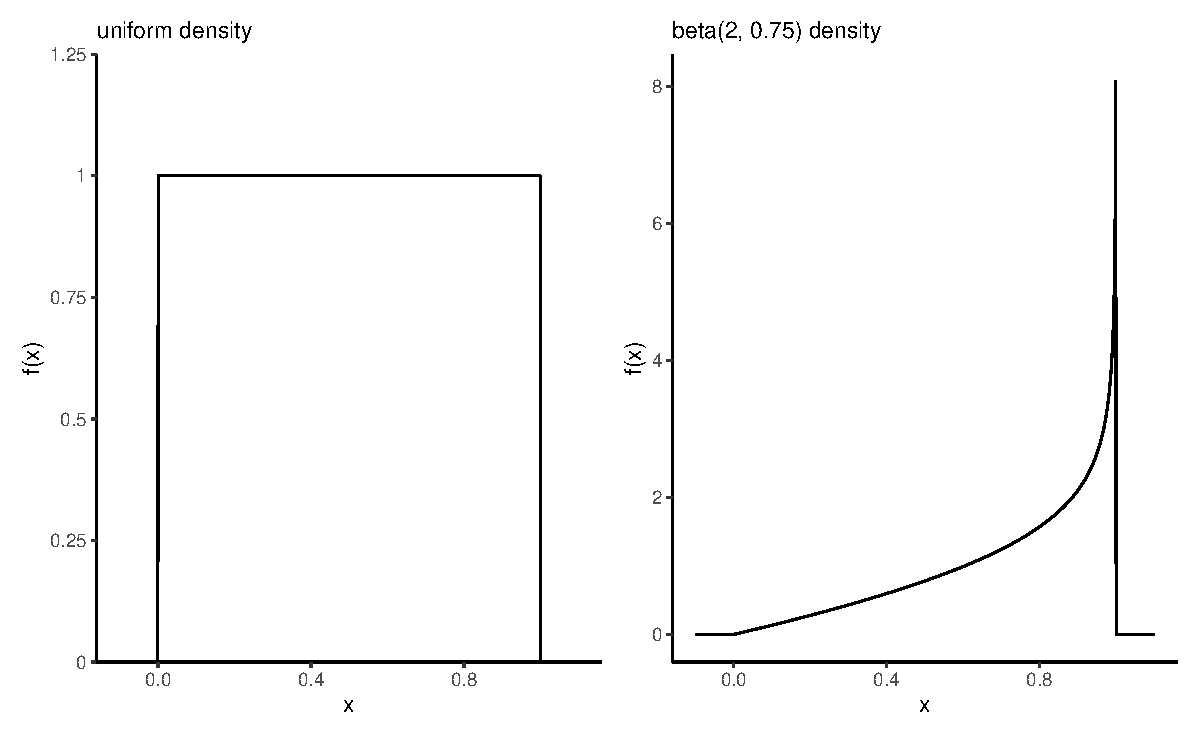
\includegraphics[width=0.85\textwidth,height=\textheight]{introduction_files/figure-pdf/fig-densite-beta-1.pdf}

}

\caption{\label{fig-densite-beta}Density fonction of uniform (left) and
beta(2, 3/4) random variables on the unit interval.}

\end{figure}%

\end{definition}

\begin{definition}[Exponential
distribution]\protect\hypertarget{def-exponentialdist}{}\label{def-exponentialdist}

The exponential distribution plays a prominent role in the study of
waiting time of Poisson processes, and in survival analysis. One
caracteristic of the distribution is it's absence of memory:
\(\Pr(Y \geq y + u \mid Y > u) = \Pr(Y > u)\) for \(y, u>0.\)

The distribution function of the exponential distribution,
\(Y \sim \mathsf{Exp}(\beta)\), here parametrized in terms of scale
\(\beta>0\) is \(F(x) = 1-\exp(-\beta x)\) and the corresponding density
function is \(f(x) =\beta\exp(-\beta x)\) for \(x >0.\) The expected
value of \(Y\) is simply \(\beta.\)

\end{definition}

\begin{definition}[Normal
distribution]\protect\hypertarget{def-normaldist}{}\label{def-normaldist}

Ths most well known distribution, the normal distribution is ubiquitous
in statistics because of the central limit theorem (CLT), which
describes the behaviour of the sample mean in large sample.The
parameters \(\mu\) and \(\sigma>0\) that fully characterize the
distribution of the normal distribution and they correspond to the
expectation and standard deviation. The density of a normal distribution
is symmetric around \(\mu\), while \(\sigma\) describes the dispersion
around this mode. The bell-shaped density function is \begin{align*}
f(x) = (2\pi\sigma^2)^{-1/2} \exp \left\{ - \frac{(x-\mu)^2}{2\sigma^2}\right\}, \qquad x \in \mathbb{R}.
\end{align*}

\begin{figure}[ht!]

\centering{

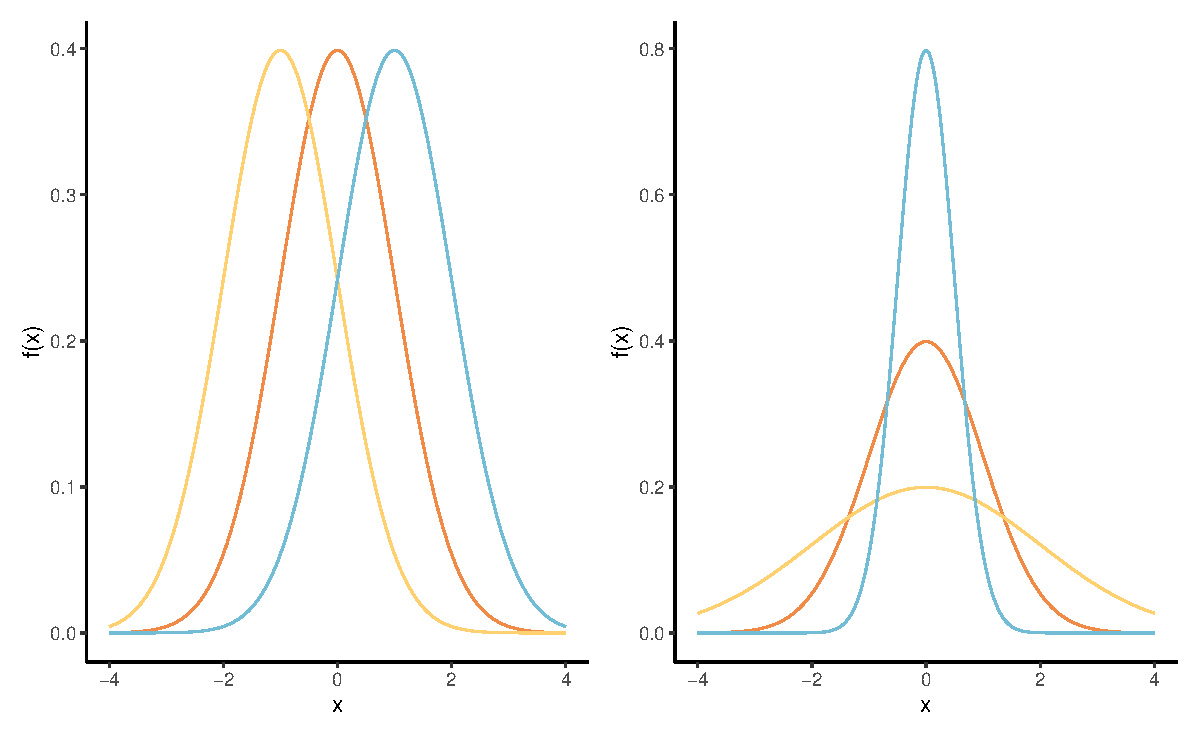
\includegraphics[width=0.85\textwidth,height=\textheight]{introduction_files/figure-pdf/fig-normal-loc-scale-1.pdf}

}

\caption{\label{fig-normal-loc-scale}Densities of normal distributions
with different mean parameters (left) and different scale parameters
(right).}

\end{figure}%

The distribution function of the normal distribution is not available in
closed-form. The normal distribution is a location-scale distribution:
if \(Y \sim \mathsf{normal}(\mu, \sigma^2)\), then
\(Z = (Y-\mu)/\sigma \sim \mathsf{normale}(0,1).\) Conversely, if
\(Z \sim \mathsf{normal}(0,1)\), then
\(Y = \mu + \sigma Z \sim \mathsf{normal}(\mu, \sigma^2).\)

We will also encounter the multivariate normal distribution; for a \(d\)
dimensional vector
\(\boldsymbol{Y} \sim \mathsf{normal}_d(\boldsymbol{\mu}, \boldsymbol{\Sigma})\),
the density is \begin{align*}
f(\boldsymbol{x}) = (2\pi)^{-d/2} |\boldsymbol{\Sigma}|^{-1/2} \exp \left\{ - \frac{1}{2} (\boldsymbol{x}-\boldsymbol{\mu})^\top \boldsymbol{\Sigma}^{-1}(\boldsymbol{x}-\boldsymbol{\mu})\right\}
\end{align*}

The mean vector \(\boldsymbol{\mu}\) is the vector of expectation of
individual observations, whereas \(\boldsymbol{\Sigma}\) is the
\(d \times d\) covariance matrix of \(\boldsymbol{Y}.\) A unique
property of the multivariate normal distribution is the link between
independence and the covariance matrix: if \(Y_i\) and \(Y_j\) are
independent, the \((i,j)\) off-diagonal entry of \(\boldsymbol{\Sigma}\)
is zero.

\end{definition}

\begin{definition}[Chi-square
distribution]\protect\hypertarget{def-chisquare-dist}{}\label{def-chisquare-dist}

The chi-square distribution with \(\nu>0\) degrees of freedom, denoted
\(\chi^2_\nu\) or \(\mathsf{chi-square}(\nu).\) It's density is
\begin{align*}
f(x; \nu) = \frac{1}{2^{\nu/2}\Gamma(\nu/2)}x^{\nu/2-1}\exp(-x/2),\qquad x >0.
\end{align*} It can be obtained for \(\nu\) integer by considering the
following: if we consider \(k\) independent and identically distributed
standard normal variables, \(Y_i \sim \mathsf{normal}(0, 1)\), then
\(\sum_{i=1}^k Y_i^2\) follows a chi-square distribution with \(k\)
degrees of freedom, denote \(\chi^2_k.\) The square of a standard normal
variate likewise follows a \(\chi^2_1\) distribution. The expectation of
\(\chi^2_k\) random variable is \(k.\)

\end{definition}

If we consider a sample of \(n\) normally distributed observations, the
scaled sample variance \((n-1)S^2/\sigma^2 \sim \chi^2_{n-1}.\)

\begin{definition}[Student-\(t\)
distribution]\protect\hypertarget{def-studentdist}{}\label{def-studentdist}

The Student-\(t\) distribution with \(\nu>0\) degrees of freedom is a
location-scale family. The standard version is denoted by
\(\mathsf{Student}(\nu).\)

The name ``Student'' comes from the pseudonym used by William Gosset in
Gosset (\citeproc{ref-Student:1908}{1908}), who introduced the
asymptotic distribution of the \(t\)-statistic. The density of the
standard \(T\) with \(\nu\) degrees of freedom is \begin{align*}
f(y; \nu) = \frac{\Gamma \left( \frac{\nu+1}{2}\right)}{\Gamma\left(\frac{\nu}{2}\right)
\sqrt{\nu\pi}}\left(1+\frac{y^{2}}{\nu}\right)^{-\frac{\nu+1}{2}}
\end{align*} the distribution has polynomial tails, is symmetric around
\(0\) and unimodal. As \(\nu \to \infty\), the Student distribution
converges to a normal distribution. It has heavier tails than the normal
distribution and only the first \(\nu-1\) moments of the distribution
exist, so a Student distribution with \(\nu=2\) degrees of freedom has
infinite variance.

For normally distributed data, the centered sample mean divided by the
sample variance, \((\overline{Y}-\mu)/S^2\) follows a Student-\(t\)
distribution with \(n-1\) degrees of freedom, which explains the
terminology \(t\)-tests.

\begin{figure}[ht!]

\centering{

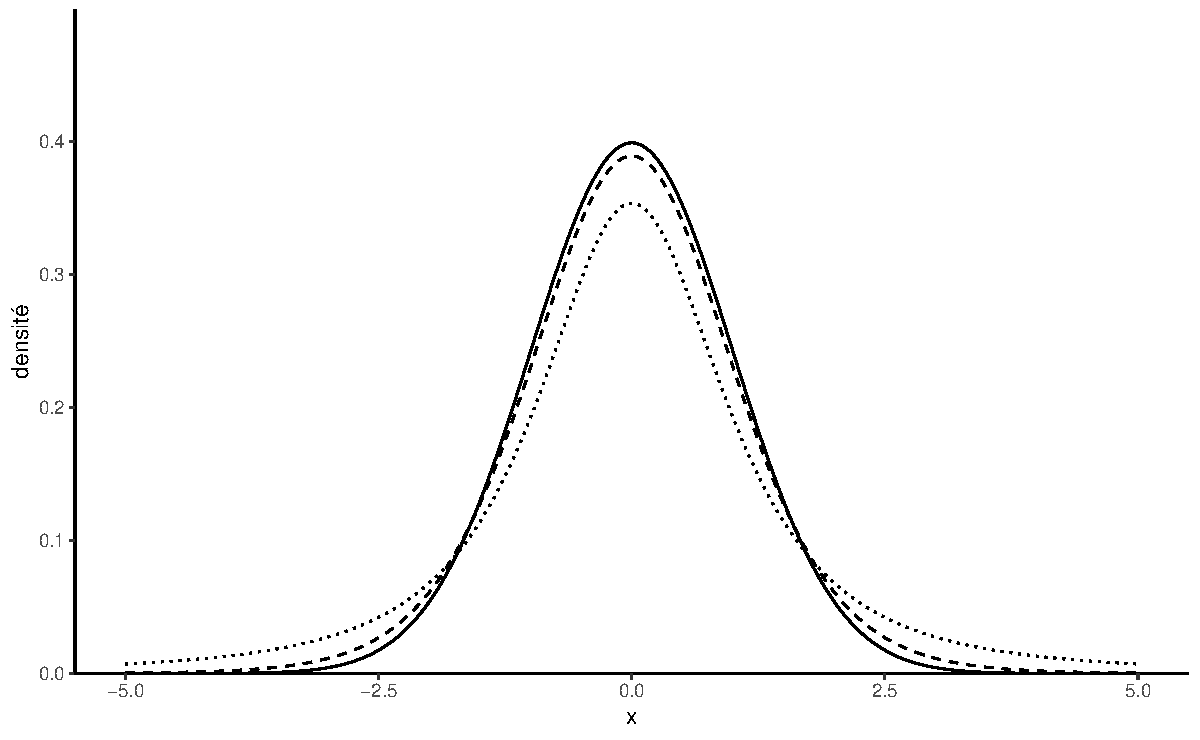
\includegraphics[width=0.5\textwidth,height=\textheight]{introduction_files/figure-pdf/fig-student-density-1.pdf}

}

\caption{\label{fig-student-density}Comparison between the Student-\(t\)
density for varying degrees of freedom, with \(\nu=2\) (dotted),
\(\nu=10\) (dashed) and the normal density (\(\nu = \infty).\)}

\end{figure}%

\end{definition}

\begin{definition}[Fisher
distribution]\protect\hypertarget{def-Fdist}{}\label{def-Fdist}

The Fisher or \(F\) distribution is used to determine the large sample
behaviour of test statistics for comparing different group averages (in
analysis of variance) assuming data are normally distributed.

The \(F\) distribution, denoted \(\mathsf{Fisher}(\nu_1, \nu_2)\), is
obtained by dividing two independent chi-square random variables with
respective degrees of freedom \(\nu_1\) and \(\nu_2.\) Specifically, if
\(Y_1 \sim \chi^2_{\nu_1}\) and \(Y_2 \sim \chi^2_{\nu_2}\), then
\begin{align*}
F = \frac{Y_1/\nu_1}{Y_2/\nu_2} \sim \mathsf{Fisher}(\nu_1, \nu_2)
\end{align*}

The Fisher distribution tends to a \(\chi^2_{\nu_1}\) when
\(\nu_2 \to \infty.\)

\end{definition}

\section{Graphs}\label{graphs}

This section reviews the main graphical representation of random
variables, depending on their type.

The main type of graph for representing categorical variables is bar
plot (and modifications thereof). In a bar plot, the frequency of each
category is represented in the \(y\)-axis as a function of the (ordered)
levels on the \(x\)-axis. This representation is superior to the
\href{http://www.perceptualedge.com/articles/08-21-07.pdf}{ignominious
pie chart}, a nuisance that ought to be banned (humans are very bad at
comparing areas and a simple rotation changes the perception of the
graph)!

\begin{figure}[ht!]

\centering{

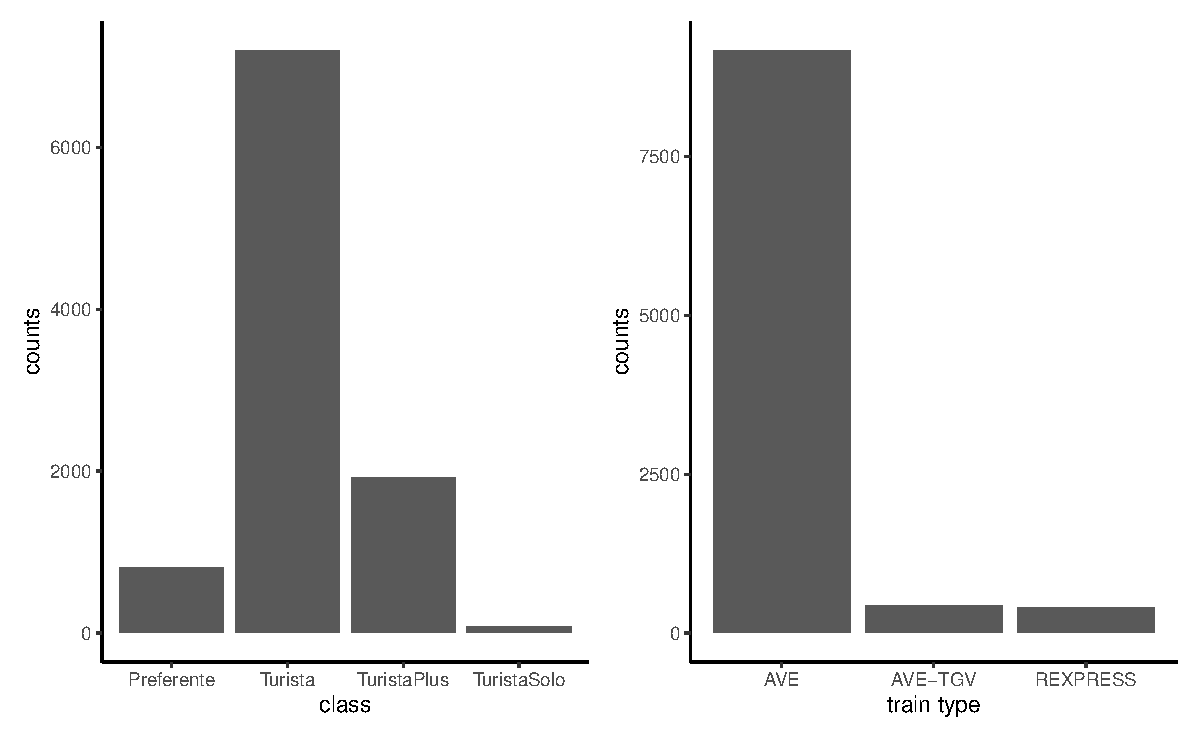
\includegraphics[width=0.85\textwidth,height=\textheight]{introduction_files/figure-pdf/fig-barplotrenfe-1.pdf}

}

\caption{\label{fig-barplotrenfe}Bar plot of ticket class for Renfe
tickets data}

\end{figure}%

Continuous variables can take as many distinct values as there are
observations, so we cannot simply count the number of occurences by
unique values. Instead, we bin them into distinct intervals so as to
obtain an histogram. The number of class depends on the number of
observations: as a rule of thumb, the number of bins should not exceed
\(\sqrt{n}\), where \(n\) is the sample size. We can then obtain the
frequency in each class, or else normalize the histogram so that the
area under the bands equals one: this yields a discrete approximation of
the underlying density function. Varying the number of bins can help us
detect patterns (rounding, asymmetry, multimodality).

Since we bin observations together, it is sometimes difficult to see
where they fall. Adding rugs below or above the histogram will add
observation about the range and values taken, where the heights of the
bars in the histogram carry information about the (relative) frequency
of the intervals.

\begin{figure}[ht!]

\centering{

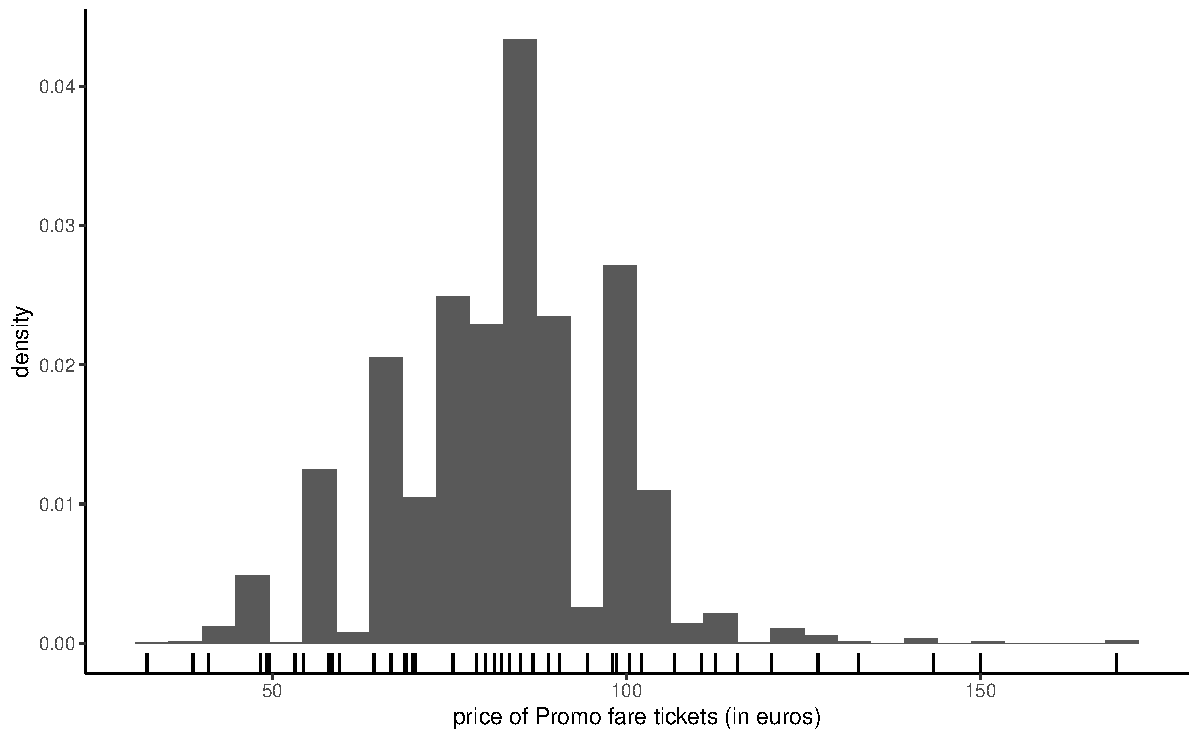
\includegraphics[width=0.85\textwidth,height=\textheight]{introduction_files/figure-pdf/fig-histrenfe-1.pdf}

}

\caption{\label{fig-histrenfe}Histogram of Promo tickets for Renfe
ticket data}

\end{figure}%

If we have a lot of data, it sometimes help to focus only on selected
summary statistics.

\begin{definition}[Box-and-whiskers
plot]\protect\hypertarget{def-boxplot}{}\label{def-boxplot}

A box-and-whiskers plot (or boxplot) represents five numbers

\begin{itemize}
\tightlist
\item
  The box gives the quartiles \(q_1, q_2, q_3\) of the distribution. The
  middle bar \(q_2\) is thus the median, so 50\% of the observations are
  smaller or larger than this number.
\item
  The length of the whiskers is up to \(1.5\) times the interquartiles
  range \(q_3-q_1\) (the whiskers extend until the latest point in the
  interval, so the largest observation that is smaller than
  \(q_3+1.5(q_3-q_1)\), etc.)
\item
  Observations beyond the whiskers are represented by dots or circles,
  sometimes termed outliers. However, beware of this terminology: the
  larger the sample size, the more values will fall outside the
  whiskers. This is a drawback of boxplots, which was conceived at a
  time where the size of data sets was much smaller than what is current
  standards.
\end{itemize}

\begin{figure}[ht!]

\centering{

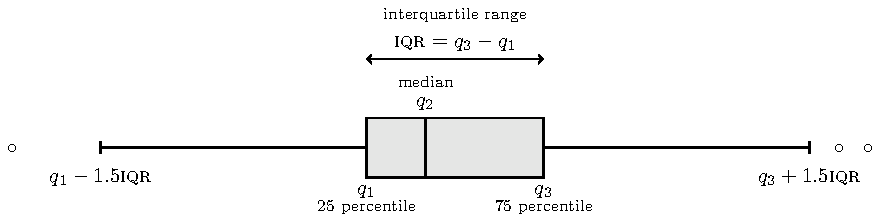
\includegraphics[width=0.85\textwidth,height=\textheight]{images/01-intro-boxplot.pdf}

}

\caption{\label{fig-boxplot}Box-and-whiskers plot}

\end{figure}%

\end{definition}

We can represent the distribution of a response variable as a function
of a categorical variable by drawing a boxplot for each category and
laying them side by side. A third variable, categorical, can be added
via a color palette, as shown in Figure~\ref{fig-histboxplot}.

\begin{figure}[ht!]

\centering{

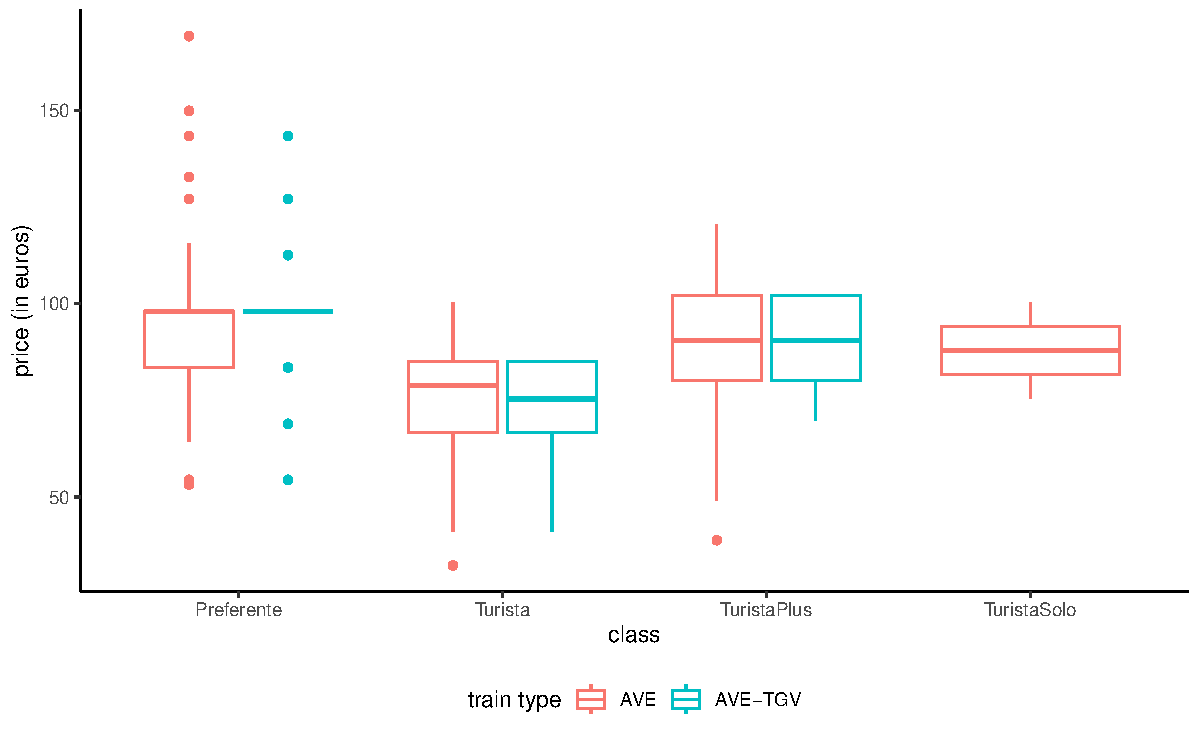
\includegraphics[width=0.85\textwidth,height=\textheight]{introduction_files/figure-pdf/fig-histboxplot-1.pdf}

}

\caption{\label{fig-histboxplot}Box-and-whiskers plots for Promo fare
tickets as a function of class and type for the Renfe tickets data.}

\end{figure}%

Scatterplots are used to represent graphically the co-variation between
two continuous variables: each tuple gives the coordinate of the point.
If only a handful of large values are visible on the graph, a
transformation may be useful: oftentimes, you will encounter graphs
where the \(x\)- or \(y\)-axis is on the log-scale when the underlying
variable is positive. If the number of data points is too large, it is
hard to distinguish points because they are overlaid: adding
transparency, or binning using a two-dimensional histogram with the
frequency represented using color are potential solutions. The left
panel of Figure~\ref{fig-scatterplot} shows the 100 simulated
observations, whereas the right-panel shows a larger sample of 10 000
points using hexagonal binning, an analog of the bivariate density.

\begin{figure}[ht!]

\centering{

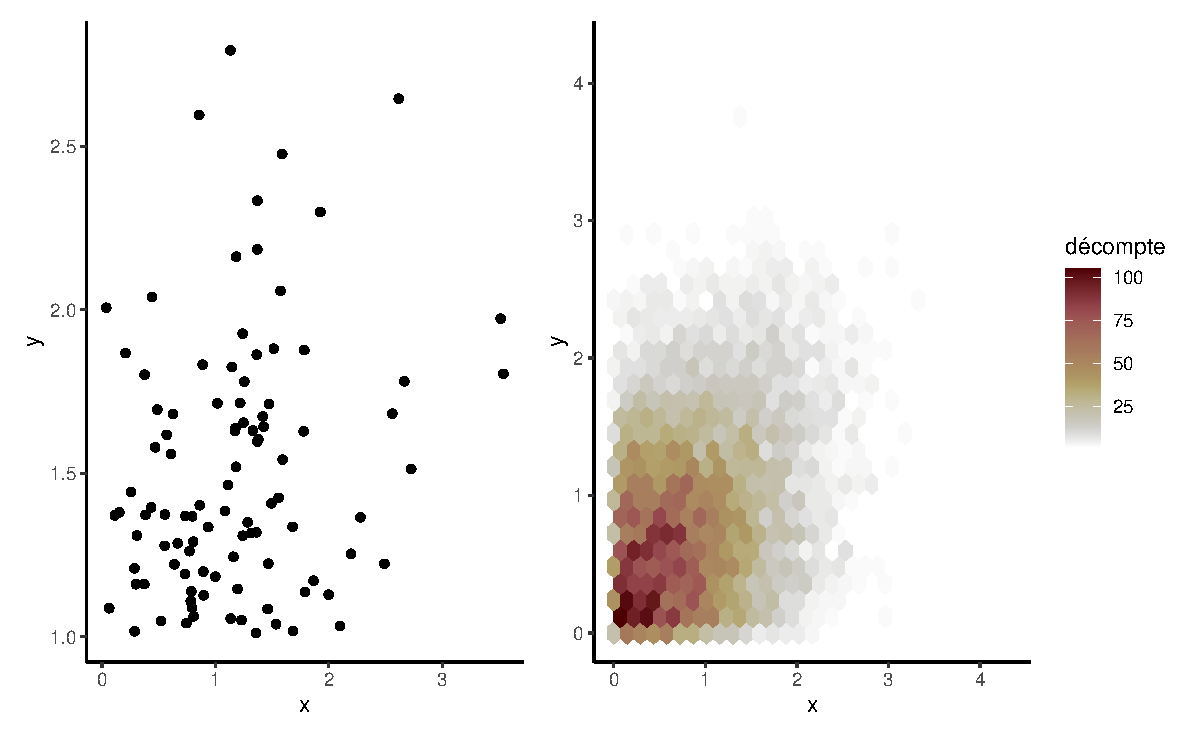
\includegraphics[width=0.85\textwidth,height=\textheight]{introduction_files/figure-pdf/fig-scatterplot-1.pdf}

}

\caption{\label{fig-scatterplot}Scatterplot (left) and hexagonal heatmap
of bidimensional bin counts (right) of simulated data.}

\end{figure}%

Models are (at best) an approximation of the true data generating
mechanism and we will want to ensure that our assumptions are reasonable
and the quality of the fit decent.

\begin{definition}[Quantiles-quantiles
plots]\protect\hypertarget{def-qqplot}{}\label{def-qqplot}

Quantile-quantile plots are graphical goodness-of-fit diagnostics that
are based on the following principle: if \(Y\) is a continuous random
variable with distribution function \(F\), then the mapping
\(F(Y) \sim \mathsf{unif}(0,1)\) yields standard uniform variables.
Similarly, the quantile transform applied to a uniform variable provides
a mean to simulating samples from \(F\), viz.~\(F^{-1}(U).\) Consider
then a random sample of size \(n\) from the uniform distribution ordered
from smallest to largest, with \(U_{(1)} \leq \cdots \leq U_{(n)}.\) One
can show these ranks have marginally a Beta distribution,
\(U_{(k)} \sim \mathsf{beta}(k, n+1-k)\) with expectation \(k/(n+1).\)

In practice, we don't know \(F\) and, even if we did, one would need to
estimate the parameters. We consider some estimator \(\widehat{F}\) for
the model and apply the inverse transform to an approximate uniform
sample \(\{i/(n+1)\}_{i=1}^n.\) The quantile-quantile plot shows the
data as a function of the (first moment) of the transformed order
statistics:

\begin{itemize}
\tightlist
\item
  on the \(x\)-axis, the theoretical quantiles
  \(\widehat{F}^{-1}\{\mathrm{rank}(y_i)/(n+1)\}\)
\item
  on the \(y\)-axis, the empirical quantiles \(y_i\)
\end{itemize}

If the model is adequate, the ordered values should follow a straight
line with unit slope passing through the origin.

\end{definition}

\begin{figure}[ht!]

\centering{

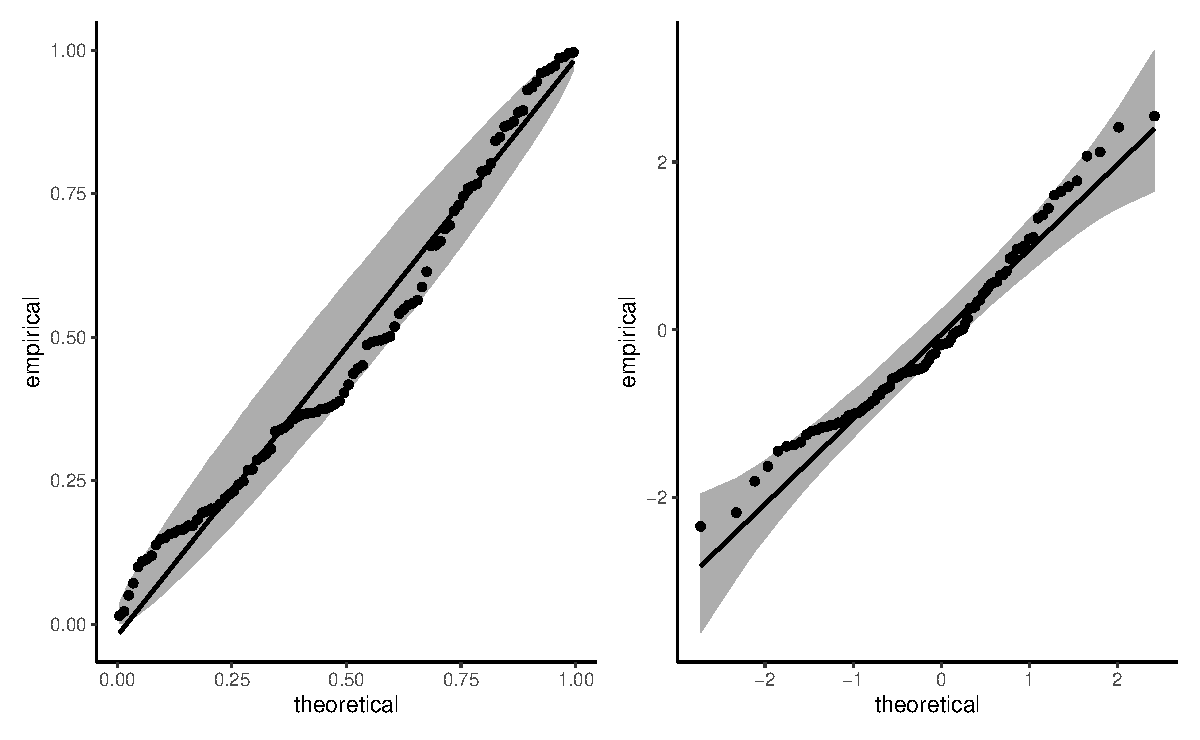
\includegraphics[width=0.85\textwidth,height=\textheight]{introduction_files/figure-pdf/fig-diagrammeqq2-1.pdf}

}

\caption{\label{fig-diagrammeqq2}Probability-probability plot (left) on
uniform margins, and ormal quantile-quantile plot (right) for the same
dataset.}

\end{figure}%

Even if we knew the true distribution of the data, the sample
variability makes it very difficult to spot if deviations from the model
are abnormal or compatible with the model. A simple point estimate with
no uncertainty measure can lead to wrong conclusions. As such, we add
approximate pointwise or simultaneous confidence intervals. The simplest
way to do this is by simulation, by repeating the following steps \(B\)
times:

\begin{enumerate}
\def\labelenumi{\arabic{enumi}.}
\tightlist
\item
  simulate a sample \(\{Y^{(b)}_{i}\} (i=1,\ldots, n)\) from
  \(\widehat{F}\)
\item
  re-estimate the parameters of \(F\) to obtain \(\widehat{F}_{(b)}\)
\item
  calculate and save the plotting positions
  \(\widehat{F}^{-1}_{(b)}\{i/(n+1)\}.\)
\end{enumerate}

The result of this operation is an \(n \times B\) matrix of simulated
data. We obtain a symmetric (\(1-\alpha\)) confidence interval by
keeping the empirical quantile of order \(\alpha/2\) and \(1-\alpha/2\)
from each row. The number \(B\) should be larger than 999, say, and be
chosen so that \(B/\alpha\) is an integer.

For the pointwise interval, each order statistic from the sample is a
statistic and so the probability of any single one falling outside the
confidence interval is approximately \(\alpha.\) However, order
statistics are not independent (they are ordered), so its common to see
neighbouring points falling outside of their respective intervals. The
intervals shown in Figure~\ref{fig-diagrammeqq2} are pointwise and
derived (magically) using a simple function. The uniform order
statistics have larger variability as we move away from 0.5, but the
uncertainty in the quantile-quantile plot largely depends on \(F.\)

Interpretation of quantile-quantile plots requires practice and
experience:
\href{https://stats.stackexchange.com/questions/101274/how-to-interpret-a-qq-plot/101290\#101290}{this
post by \emph{Glen\_b} on StackOverflow} nicely summarizes what can be
detected (or not) from them.

\section{Laws of large numbers}\label{law-large-numbers}

An estimator for a parameter \(\theta\) is \textbf{consistent} if the
value obtained as the sample size increases (to infinity) converges to
the true value of \(\theta.\) Mathematically speaking, this translates
into convergence in probability, meaning
\(\hat{\theta} \stackrel{\mathsf{Pr}}{\to} \theta.\) In common language,
we say that the probability that \(\hat{\theta}\) and \(\theta\) differ
becomes negligible as \(n\) gets large.

Consistency is the \emph{a minima} requirement for an estimator: when we
collect more information, we should approach the truth. The law of large
number states that the sample mean of \(n\) (independent) observations
with common mean \(\mu\), say \(\overline{Y}_n\), converges to \(\mu\),
denoted \(\overline{Y}_n \rightarrow \mu.\) Roughly speaking, our
approximation becomes less variable and asymptotically unbiased as the
sample size (and thus the quantity of information available for the
parameter) increases. The law of large number is featured in Monte Carlo
experiments: we can approximate the expectation of some (complicated)
function \(g(x)\) by simulating repeatedly independent draws from \(Y\)
and calculating the sample mean \(n^{-1} \sum_{i=1}^n g(Y_i).\)

If the law of large number tells us what happens in the limit (we get a
single numerical value), the result doesn't contain information about
the rate of convergence and the uncertainty at finite levels.

\section{Central Limit Theorem}\label{CLT}

The central limit theorem gives the approximate large sample
distribution of the sample mean. Consider a random sample of size \(n\)
\(\{Y_i\}_{i=1}^n\) of independent random variables with common
expectation \(\mu\) and variance \(\sigma^2.\) The sample mean
\(\overline{Y} = n^{-1}\sum_{i=1}^n Y_i\) converges to \(\mu\) by the
law of large number, but we also have that

\begin{itemize}
\tightlist
\item
  the estimator \(\overline{Y}\) is centered around \(\mu\),
\item
  the standard error is \(\sigma/\sqrt{n}\); the rate of convergence is
  thus \(\sqrt{n}.\) For a sample of size 100, the standard error of the
  sample mean will be 10 times smaller than that of the underlying
  random variable.
\item
  the sample mean, once properly scaled, follows approximately a normal
  distribution
\end{itemize}

Mathematically, the central limit theorem states
\(\sqrt{n}(\overline{Y}-\mu) \stackrel{\mathrm{d}}{\rightarrow} \mathsf{normal}(0, \sigma^2).\)
If \(n\) is large (a rule of thumb is \(n>30\), but this depends on the
underlying distribution of \(Y\)), then
\(\overline{Y} \stackrel{\cdot}{\sim} \mathsf{normal}(\mu, \sigma^2/n).\)

How do we make sense of this result? Let us consider the mean travel
time of high speed Spanish trains (AVE) between Madrid and Barcelona
that are operated by Renfe.

\begin{figure}[ht!]

\centering{

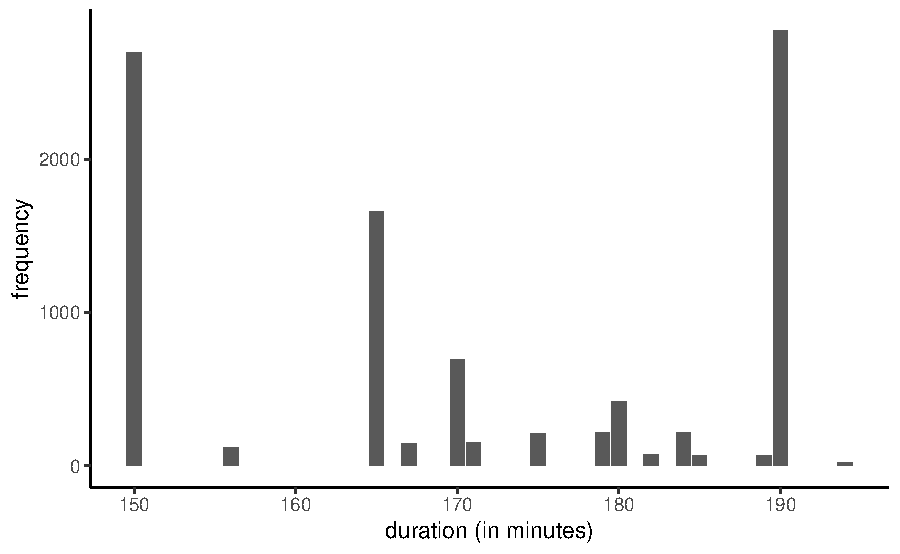
\includegraphics[width=0.85\textwidth,height=\textheight]{introduction_files/figure-pdf/fig-renfeclt-1.pdf}

}

\caption{\label{fig-renfeclt}Empirical distribution of travel times of
high speed trains.}

\end{figure}%

Our exploratory data analysis showed previously that the duration is the
one advertised on the ticket: there are only 15 unique travel time.
Based on 9603 observations, we estimate the mean travel time to be 170
minutes and 41 seconds. Figure~\ref{fig-renfeclt} shows the empirical
distribution of the data.

Consider now samples of size \(n=10\), drawn repeatedly from the
population: in the first sample, the sample mean is 169.3 minutes,
whereas we get an estimate of 167 minutes in our second , 157.9 minutes
in the third, etc.

\begin{figure}[ht!]

\centering{

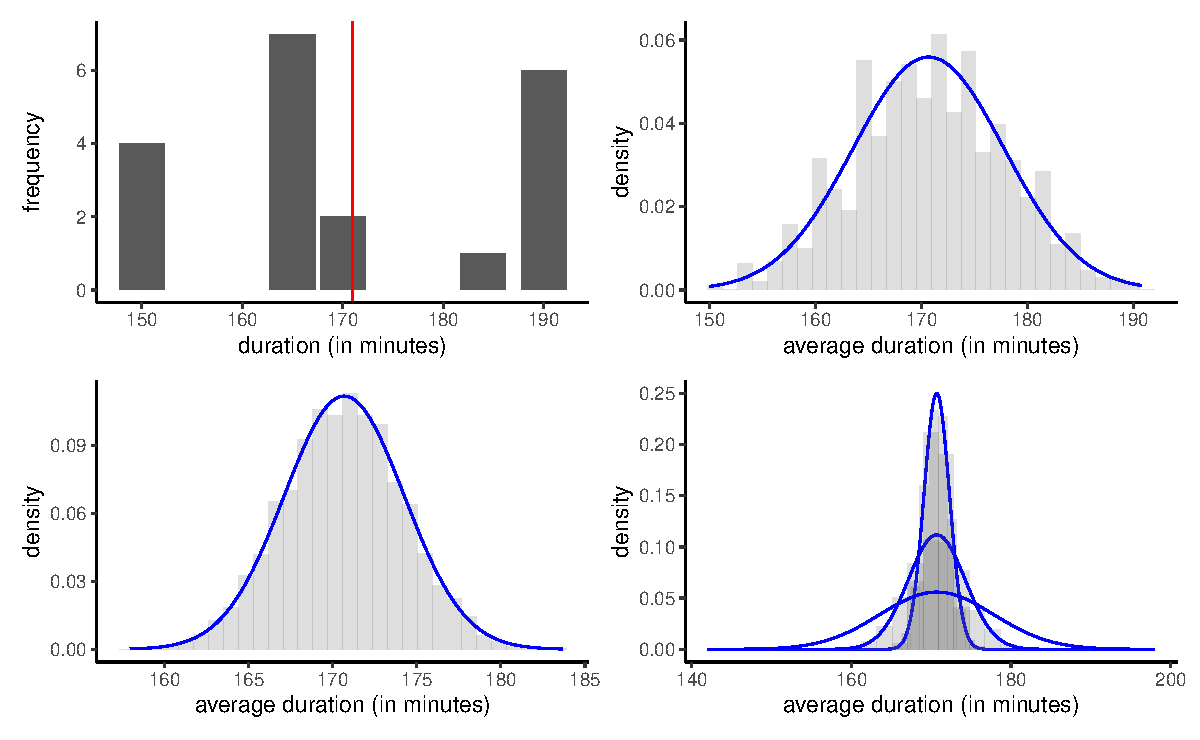
\includegraphics[width=0.9\textwidth,height=\textheight]{introduction_files/figure-pdf/fig-renfemeanCLT-1.pdf}

}

\caption{\label{fig-renfemeanCLT}Graphical representation of the central
limit theorem. The upper left panel shows a sample of 20 observations
with its sample mean (vertical red). The three other panels show the
histograms of the sample mean from repeated samples of size 5 (top
right), 20 (bottom left) and 20, 50 and 100 overlaid, with the density
approximation provided by the central limit theorem.}

\end{figure}%

We draw \(B=1000\) different samples, each of size \(n=5\), from two
millions records, and calculate the sample mean in each of them. The top
right panel of Figure~\ref{fig-renfemeanCLT} is a histogram of the
sample means when \(n=5\), whereas the bottom left panel shows the same
thingfor \(n=20.\) The last graph of Figure~\ref{fig-renfemeanCLT} shows
the impact of the increase in sample size: whereas the normal
approximation is okay-ish for \(n=5\), it is indistinguishable from the
normal approximation for \(n=20.\) As \(n\) increases and the sample
size gets bigger, the quality of the approximation improves and the
curve becomes more concentrated around the true mean. Even if the
distribution of the travel time is discrete, the mean is approximately
normal.

We considered a single distribution in the example, but you could play
with other distributions and vary the sample size to see when the
central limit theorem kicks in usng this
\href{http://195.134.76.37/applets/AppletCentralLimit/Appl_CentralLimit2.html}{applet}.

The central limit theorem underlies why scaled test statistics which
have sample mean zero and sample variance 1 have a standard null
distribution in large sample: this is what guarantees the validity of
our inference!

\bookmarksetup{startatroot}

\chapter{Statistical inference}\label{inference}

In most applied domains, empirical evidences drive the advancement of
the field and data from well designed experiments contribute to the
built up of science. In order to draw conclusions in favour or against a
theory, researchers turn (often unwillingly) to statistics to back up
their claims. This has led to the prevalence of the use of the null
hypothesis statistical testing (NHST) framework. One important aspect of
the reproducibility crisis is the misuse of \(p\)-values in journal
articles: falsification of a null hypothesis is not enough to provide
substantive findings for a theory.

Because introductory statistics course typically present hypothesis
tests without giving much thoughts to the underlying construction
principles of such procedures, users often have a reductive view of
statistics as a catalogue of pre-determined procedures. To make a
culinary analogy, users focus on learning recipes rather than trying to
understand the basics of cookery. This chapter focuses on understanding
of key ideas related to testing.

\begin{tcolorbox}[enhanced jigsaw, colframe=quarto-callout-important-color-frame, title=\textcolor{quarto-callout-important-color}{\faExclamation}\hspace{0.5em}{Important}, opacityback=0, leftrule=.75mm, colbacktitle=quarto-callout-important-color!10!white, breakable, bottomrule=.15mm, toprule=.15mm, toptitle=1mm, opacitybacktitle=0.6, left=2mm, bottomtitle=1mm, colback=white, arc=.35mm, coltitle=black, titlerule=0mm, rightrule=.15mm]

\textbf{Learning objectives}:

\begin{itemize}
\tightlist
\item
  Understanding the role of uncertainty in decision making.
\item
  Understanding the importance of signal-to-noise ratio as a measure of
  evidence.
\item
  Knowing the basic ingredients of hypothesis testing and being capable
  of correctly formulating and identifying these components in a paper.
\item
  Correctly interpreting \(p\)-values and confidence intervals for a
  parameter.
\end{itemize}

\end{tcolorbox}

The first step of a design is formulating a research question.
Generally, this hypothesis will specify potential differences between
population characteristics due to some intervention (a treatment) that
the researcher wants to quantify. This is the step during which
researchers decide on sample size, choice of response variable and
metric for the measurement, write down the study plan, etc.

It is important to note that most research questions cannot be answered
by simple tools. Researchers wishing to perform innovative
methodological research should contact experts and consult with
statisticians \textbf{before} they collect their data to get information
on how best to proceed for what they have in mind so as to avoid the
risk of making misleading and false claims based on incorrect analysis
or data collection.

\begin{figure}[ht!]

\centering{

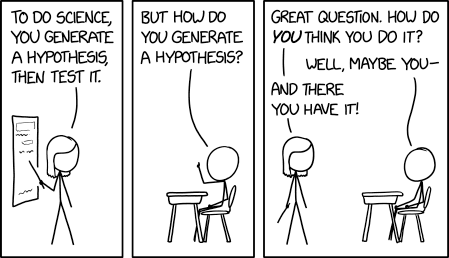
\includegraphics[width=0.6\textwidth,height=\textheight]{images/xkcd2569_hypothesis_generation.png}

}

\caption{\label{fig-xkcd2569}xkcd comic
\href{https://xkcd.com/2569/}{2569 (Hypothesis generation) by Randall
Munroe}. Alt text: Frazzled scientists are requesting that everyone
please stop generating hypotheses for a little bit while they work
through the backlog. Cartoon reprinted under the
\href{https://creativecommons.org/licenses/by-nc/2.5/}{CC BY-NC 2.5
license}.}

\end{figure}%

\section{Sampling variability}\label{sampling-variability}

Given data, a researcher will be interested in estimating particular
characteristics of the population. We can characterize the set of all
potential values their measurements can take, together with their
frequency, via a distribution.

The purpose of this section is to illustrate how we cannot simply use
raw differences between groups to make meaningful comparisons: due to
sampling variability, samples will be alike even if they are generated
in the same way, but there will be always be differences between their
summary statistics. Such differences tend to attenuate (or increase) as
we collect more sample. Inherent to this is the fact that as we gather
more data (and thus more information) about our target, the portrait
becomes more precise. This is ultimately what allows us to draw
meaningful conclusions but, in order to do so, we need first to
determine what is likely or plausible and could be a stroke of luck, and
what is not likely to occur solely due to randomness.

We call numerical summaries of the data \textbf{statistics}. Its
important to distinguish between procedures/formulas and their numerical
values. An \textbf{estimator} is a rule or formula used to calculate an
estimate of some parameter or quantity of interest based on observed
data (like a recipe for cake). Once we have observed data we can
actually compute the sample mean, that is, we have an estimate --- an
actual value (the cake), which is a single realization and not random.
In other words,

\begin{itemize}
\tightlist
\item
  an estimand is our conceptual target, like the population
  characteristic of interest (population mean).
\item
  an estimator is the procedure or formula telling us how to transform
  the sample data into a numerical summary that is a proxy of our
  target.
\item
  an estimate is a number, the numerical value obtained once we apply
  the formula to observed data.
\end{itemize}

\begin{figure}[ht!]

\begin{minipage}{0.33\linewidth}

\centering{


\includegraphics[width=0.85\textwidth,height=\textheight]{images/estimand.jpg}

}

\subcaption{\label{fig-cake-1}Estimand}

\end{minipage}%
%
\begin{minipage}{0.33\linewidth}

\centering{

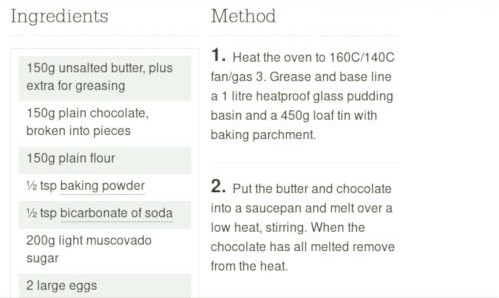
\includegraphics[width=0.85\textwidth,height=\textheight]{images/estimator.jpg}

}

\subcaption{\label{fig-cake-2}Estimator}

\end{minipage}%
%
\begin{minipage}{0.33\linewidth}

\centering{


\includegraphics[width=0.85\textwidth,height=\textheight]{images/estimate.jpg}

}

\subcaption{\label{fig-cake-3}Estimate}

\end{minipage}%

\caption{\label{fig-cake}\href{https://www.flickr.com/photos/darkdwarf/16563489881}{Estimand}
(left), estimator (middle) and
\href{https://www.flickr.com/photos/bensutherland/14685548773}{estimate}
(right) illustrated with cakes and based on an original idea of Simon
Grund. Cake photos shared under
\href{https://creativecommons.org/licenses/by-nc/2.0/}{CC BY-NC 2.0
license}.}

\end{figure}%

For example, we may use as estimand the population average of
\(Y_1, \ldots,\) say \(\mu.\) The estimator will be sample mean, i.e.,
the sum of the elements in the sample divided by the sample size,
\(\overline{Y}=(Y_1 + \cdots + Y_n)/n.\) The estimate will be a
numerical value, say 4.3.

Because the inputs of the estimator are random, the output is also
random and change from one sample to the next: even if you repeat a
recipe, you won't get the exact same result every time, as in
Figure~\ref{fig-xkcd605}.

\begin{figure}[ht!]

\centering{

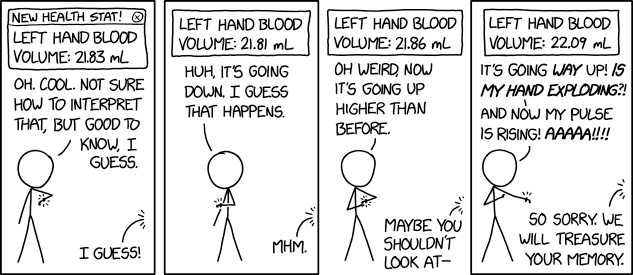
\includegraphics[width=0.7\textwidth,height=\textheight]{images/xkcd2581_health_stats.png}

}

\caption{\label{fig-xkcd605}xkcd comic
\href{https://xkcd.com/2581/}{2581 (Health Stats) by Randall Munroe}.
Alt text: You will live on forever in our hearts, pushing a little extra
blood toward our left hands now and then to give them a squeeze. Cartoon
reprinted under the
\href{https://creativecommons.org/licenses/by-nc/2.5/}{CC BY-NC 2.5
license}.}

\end{figure}%

To illustrate this point, Figure~\ref{fig-samplevar} shows five simple
random samples of size \(n=10\) drawn from an hypothetical population
with mean \(\mu\) and standard deviation \(\sigma,\) along with their
sample mean \(\overline{y}.\) Because of the sampling variability, the
sample means of the subgroups will differ even if they originate from
the same distribution. You can view sampling variability as noise: our
goal is to extract the signal (typically differences in means) but
accounting for spurious results due to the background noise.

\begin{figure}[ht!]

\centering{

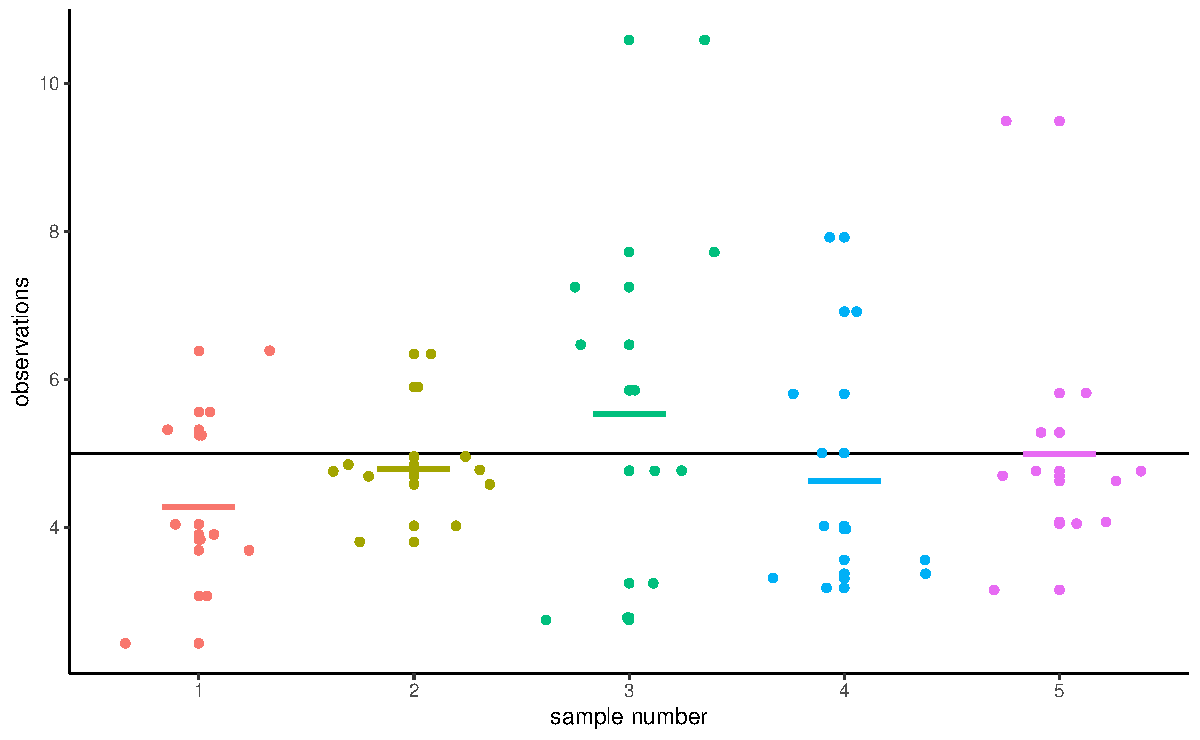
\includegraphics[width=0.85\textwidth,height=\textheight]{inference_files/figure-pdf/fig-samplevar-1.pdf}

}

\caption{\label{fig-samplevar}Five samples of size \(n=10\) drawn from a
common population with mean \(\mu\) (horizontal line). The colored
segments show the sample means of each sample.}

\end{figure}%

The astute eye might even notice that the sample means (thick horizontal
segments) are less dispersed around the full black horizontal line
representing the population average \(\mu\) than are the individual
measurements. This is a fundamental principle of statistics: information
accumulates as you get more data.

Values of the sample mean don't tell the whole picture and studying
differences in mean (between groups, or relative to a postulated
reference value) is not enough to draw conclusions. In most settings,
there is no guarantee that the sample mean will be equal to it's true
value because it changes from one sample to the next: the only guarantee
we have is that it will be on average equal to the population average in
repeated samples. Depending on the choice of measurement and variability
in the population, there may be considerable differences from one
observation to the next and this means the observed difference could be
a fluke.

To get an idea of how certain something is, we have to consider the
variability of an observation \(Y_i.\) This variance of an observation
drawn from the population is typically denoted \(\sigma^2\) and it's
square root, the standard deviation, by \(\sigma.\)

The standard deviation \emph{of a statistic} is termed \textbf{standard
error}; it should not be confused with the standard deviation \(\sigma\)
of the population from which the sample observations
\(Y_1, \ldots, Y_n\) are drawn. Both standard deviation and standard
error are expressed in the same units as the measurements, so are easier
to interpret than variance. Since the standard error is a function of
the sample size, it is however good practice to report the estimated
standard deviation in reports.

\begin{example}[Sample proportion and uniform
draws]\protect\hypertarget{exm-samppropunif}{}\label{exm-samppropunif}

To illustrate the concept of sampling variability, we follow the lead of
\href{https://www.crumplab.com/statistics/foundations-for-inference.html}{Matthew
Crump} and consider samples from a uniform distribution on
\(\{1, 2, \ldots, 10\}\) each number in this interval is equally likely
to be sampled.

\begin{figure}[ht!]

\centering{

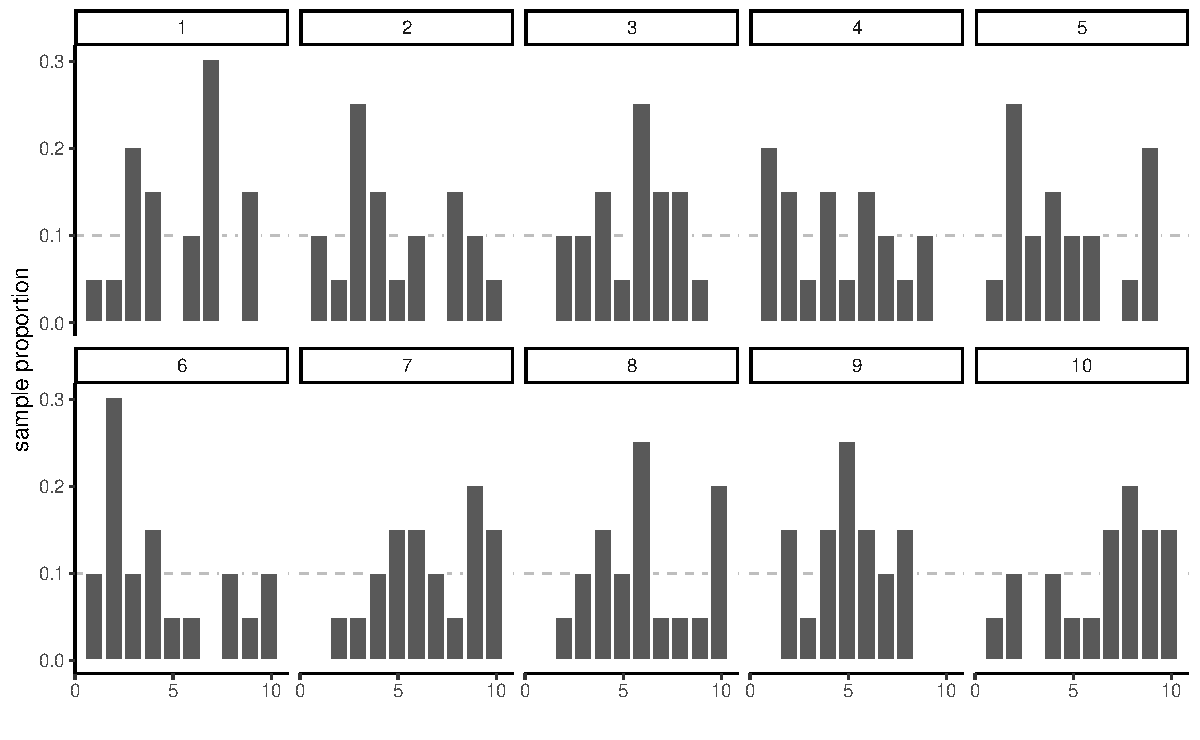
\includegraphics[width=0.85\textwidth,height=\textheight]{inference_files/figure-pdf/fig-unifsamp1-1.pdf}

}

\caption{\label{fig-unifsamp1}Histograms for 10 random samples of size
\(n=20\) from a discrete uniform distribution.}

\end{figure}%

Even if they are drawn from the same population, the 10 samples in
Figure~\ref{fig-unifsamp1} look quite different. The only thing at play
here is the sample variability: since there are \(n=20\) observations in
total, there should be on average 10\% of the observations in each of
the 10 bins, but some bins are empty and others have more counts than
expected. This fluctuation is due to randomness, or chance.

How can we thus detect whether what we see is compatible with the model
we think generated the data? The key is to collect more observations:
the bar height is the sample proportion, an average of 0/1 values with
ones indicating that the observation is in the bin and zero otherwise.

Consider now what happens as we increase the sample size: the top panel
of Figure~\ref{fig-uniformsamp2} shows uniform samples for increasing
samples size. The scaled bar plot looks more and more like the true
underlying distribution (flat, each bin with equal frequency) as the
sample size increases. The sample distribution of points is nearly
indistinguishable from the theoretical one (straight line) when
\(n=10 000.\)\footnote{The formula shows that the standard error
  decreases by a tenfold every time the sample size increases by a
  factor 100.} The bottom panel, on the other hand, isn't from a uniform
distribution and larger samples come closer to the population
distribution. We couldn't have spotted this difference in the first two
plots, since the sampling variability is too important; there, the lack
of data in some bins could have been attributed to chance, as they are
comparable with the graph for data that are truly uniform. This is in
line with most practical applications, in which the limited sample size
restricts our capacity to disentangle real differences from sampling
variability. We must embrace this uncertainty: in the next section, we
outline how hypothesis testing helps us disentangle the signal from the
noise.

\begin{figure}[ht!]

\centering{

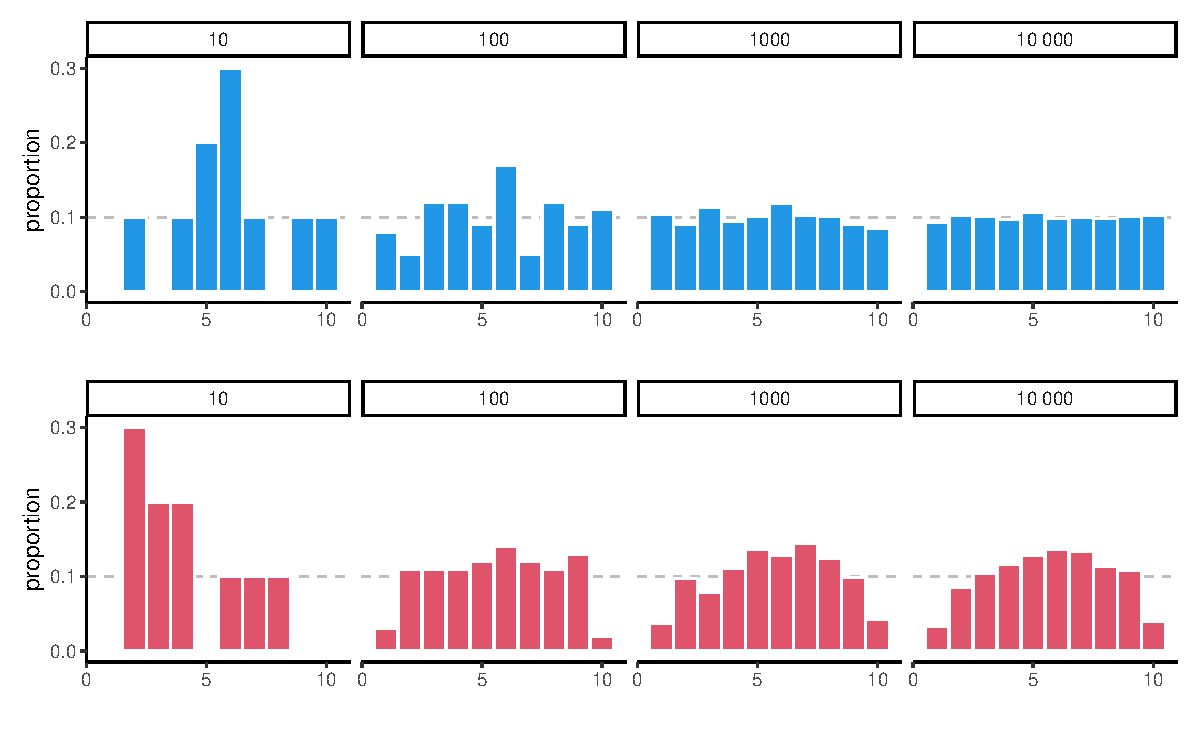
\includegraphics[width=0.85\textwidth,height=\textheight]{inference_files/figure-pdf/fig-uniformsamp2-1.pdf}

}

\caption{\label{fig-uniformsamp2}Bar plots of data from a uniform
distribution (top) and non-uniform (bottom) with increasing sample sizes
of 10, 100, 1000 and 10 000 (from left to right).}

\end{figure}%

\end{example}

\section{Hypothesis testing}\label{tests}

An \textbf{hypothesis test} is a binary decision rule used to evaluate
the statistical evidence provided by a sample to make a decision
regarding the underlying population. The main steps involved are:

\begin{itemize}
\tightlist
\item
  define the model parameters
\item
  formulate the alternative and null hypothesis
\item
  choose and calculate the test statistic
\item
  obtain the null distribution describing the behaviour of the test
  statistic under \(\mathscr{H}_0\)
\item
  calculate the \emph{p}-value
\item
  conclude (reject or fail to reject \(\mathscr{H}_0\)) in the context
  of the problem.
\end{itemize}

A good analogy for hypothesis tests is a trial for murder on which you
are appointed juror.

\begin{itemize}
\tightlist
\item
  The judge lets you choose between two mutually exclusive outcome,
  guilty or not guilty, based on the evidence presented in court.
\item
  The presumption of innocence applies and evidences are judged under
  this optic: are evidence remotely plausible if the person was
  innocent? The burden of the proof lies with the prosecution to avoid
  as much as possible judicial errors. The null hypothesis
  \(\mathscr{H}_0\) is \emph{not guilty}, whereas the alternative
  \(\mathscr{H}_a\) is \emph{guilty}. If there is a reasonable doubt,
  the verdict of the trial will be not guilty.
\item
  The test statistic (and the choice of test) represents the summary of
  the proof. The more overwhelming the evidence, the higher the chance
  the accused will be declared guilty. The prosecutor chooses the proof
  so as to best outline this: the choice of evidence (statistic)
  ultimately will maximise the evidence, which parallels the power of
  the test.
\item
  The final step is the verdict. This is a binary decision, guilty or
  not guilty. For an hypothesis test performed at level \(\alpha,\) one
  would reject (guilty) if the \emph{p}-value is less than \(\alpha.\)
\end{itemize}

The above description provides some heuristic, but lacks crucial
details.

\section{Hypothesis}\label{hypothesis}

In statistical tests we have two hypotheses: the null hypothesis
(\(\mathscr{H}_0\)) and the alternative hypothesis (\(\mathscr{H}_1\)).
Usually, the null hypothesis is the `status quo' and the alternative is
what we're really interested in testing. A statistical hypothesis test
allows us to decide whether or not our data provides enough evidence to
reject \(\mathscr{H}_0\) in favour of \(\mathscr{H}_1,\) subject to some
pre-specified risk of error. Usually, hypothesis tests involve a
parameter, say \(\theta,\) which characterizes the underlying
distribution at the population level ans whose value is unknown. A
two-sided hypothesis test regarding a parameter \(\theta\) has the form
\begin{align*}
\mathscr{H}_0: \theta=\theta_0 \qquad \text{versus} \qquad \mathscr{H}_a:\theta \neq \theta_0.
\end{align*} We are testing whether or not \(\theta\) is precisely equal
to the value \(\theta_0.\) The hypotheses are a statistical
representation of our research question.

A common example of two-sided test is one for the regression coefficient
\(\beta_j\) associated to an explanatory variable \(\mathrm{X}_j,\) for
which the null and alternative hypothesis are \begin{align*}
\mathscr{H}_0: \beta_j=\beta_j^0 \qquad \text{versus} \qquad \mathscr{H}_a:\beta_j \neq \beta_j^0,
\end{align*} where \(\beta_j^0\) is some value that reflects the
research question of interest. For example, if \(\beta_j^0=0,\) the
underlying question is: is covariate \(\mathrm{X}_j\) impacting the
response \(Y\) linearly once other variables have been taken into
account?

Note that we can impose direction in the hypotheses and consider
alternatives of the form \(\mathscr{H}_a: \theta > \theta_0\) or
\(\mathscr{H}_a: \theta < \theta_0.\)

\section{Test statistic}\label{test-statistic}

A test statistic \(T\) is a function of the data that summarise the
information contained in the sample for \(\theta.\) The form of the test
statistic is chosen such that we know its underlying distribution under
\(\mathscr{H}_0,\) that is, the potential values taken by \(T\) and
their relative probability if \(\mathscr{H}_0\) is true. Indeed, \(Y\)
is a random variable and its value change from one sample to the next.
This allows us to determine what values of \(T\) are likely if
\(\mathscr{H}_0\) is true. Many statistics we will consider are
\textbf{Wald statistic}, of the form \begin{align*}
T = \frac{\widehat{\theta} - \theta_0}{\mathrm{se}(\widehat{\theta})}
\end{align*} where \(\widehat{\theta}\) is an estimator of \(\theta,\)
\(\theta_0\) is the postulated value of the parameter and
\(\mathrm{se}(\widehat{\theta})\) is an estimator of the standard
deviation of the test statistic \(\widehat{\theta}.\)

For example, to test whether the mean of a population is zero, we set
\begin{align*}
\mathscr{H}_0: \mu=0, \qquad  \mathscr{H}_a:\mu \neq 0,
\end{align*} and the Wald statistic is \begin{align*}
T &= \frac{\overline{X}-0}{S_n/\sqrt{n}}
\end{align*} where \(\overline{X}\) is the sample mean of
\(X_1, \ldots, X_n,\) \begin{align*}
\overline{X} &= \frac{1}{n} \sum_{i=1}^n X_i = \frac{X_1+ \cdots + X_n}{n}
\end{align*} and the standard error (of the mean) \(\overline{X}\) is
\(S_n/\sqrt{n}\); the sample variance \(S_n\) is an estimator of the
standard deviation \(\sigma,\) \begin{align*}
S^2_n &= \frac{1}{n-1} \sum_{i=1}^n (X_i-\overline{X})^2.
\end{align*}

\section{\texorpdfstring{Null distribution and
\emph{p}-value}{Null distribution and p-value}}\label{null-distribution-and-p-value}

The \emph{p}-value allows us to decide whether the observed value of the
test statistic \(T\) is plausible under \(\mathscr{H}_0.\) Specifically,
the \emph{p}-value is the probability that the test statistic is equal
or more extreme to the estimate computed from the data, assuming
\(\mathscr{H}_0\) is true. Suppose that based on a random sample
\(Y_1, \ldots, Y_n\) we obtain a statistic whose value \(T=t.\) For a
two-sided test \(\mathscr{H}_0:\theta=\theta_0\)
vs.~\(\mathscr{H}_a:\theta \neq \theta_0,\) the \emph{p}-value is
\(\Pr_0(|T| \geq |t|).\)\footnote{If the distribution of \(T\) is
  symmetric around zero, the \emph{p}-value reduces to
  \(p = 2 \times \Pr_0(T \geq |t|).\)}

How do we determine the null distribution given that the true data
generating mechanism is unknown to us? We ask a statistician! In simple
cases, it might be possible to enumerate all possible outcomes and thus
quantity the degree of outlyingness of our observed statistic. In more
general settings, we can resort to simulations or to probability theory:
the central limit theorem says that the sample mean behaves like a
normal random variable with mean \(\mu\) and standard deviation
\(\sigma/\sqrt{n}\) for \(n\) large enough. The central limit theorem
has broader applications since most statistics can be viewed as some
form of average or transformation thereof, a fact used to derive
benchmarks for most commonly used tests. Most software use these
approximations as proxy by default: the normal, Student's \(t,\)
\(\chi^2\) and \(F\) distributions are the reference distributions that
arise the most often.

Figure~\ref{fig-power-plots} shows the distribution of \(p\)-values for
two scenarios: one in which there are no differences and the null is
true, the other under an alternative. The probability of rejection is
obtained by calculating the area under the density curve between zero
and \(\alpha=0.1,\) here 0.1 on the left. Under the null, the model is
calibrated and the distribution of \emph{p}-values is uniform (i.e., a
flat rectangle of height 1), meaning all values in the unit interval are
equally likely. Under the alternative (right), small \emph{p}-values are
more likely to be observed.

\begin{figure}[ht!]

\centering{

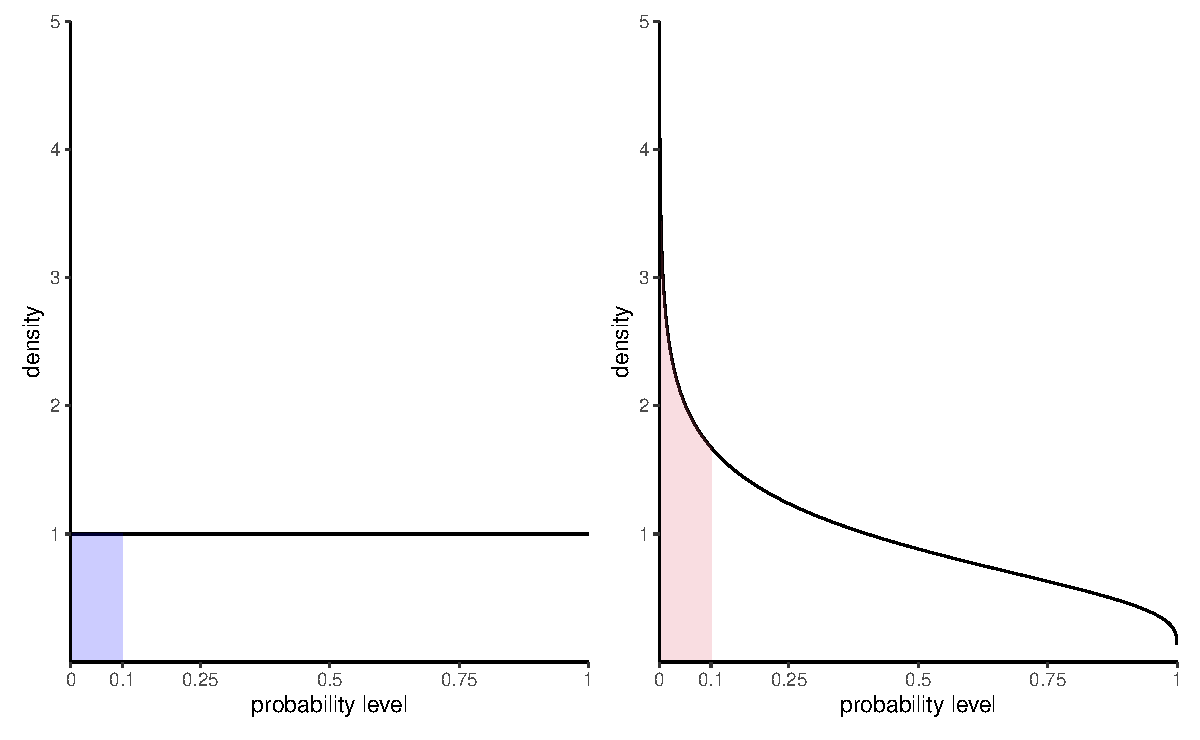
\includegraphics[width=0.85\textwidth,height=\textheight]{inference_files/figure-pdf/fig-power-plots-1.pdf}

}

\caption{\label{fig-power-plots}Density of \emph{p}-values under the
null hypothesis (left) and under an alternative with a signal-to-noise
ratio of 0.5 (right).}

\end{figure}%

There are generally three ways of obtaining null distributions for
assessing the degree of evidence against the null hypothesis

\begin{itemize}
\tightlist
\item
  exact calculations
\item
  large sample theory (aka `asymptotics' in statistical lingo)
\item
  simulation
\end{itemize}

While desirable, the first method is only applicable in simple cases
(such as counting the probability of getting two six if you throw two
fair die). The second method is most commonly used due to its generality
and ease of use (particularly in older times where computing power was
scarce), but fares poorly with small sample sizes (where `too small' is
context and test-dependent). The last approach can be used to
approximate the null distribution in many scenarios, but adds a layer of
randomness and the extra computations costs sometimes are not worth it.

Consider the example of a two-sided test involving the population mean
\(\mathscr{H}_0:\mu=0\) against the alternative
\(\mathscr{H}_1:\mu \neq 0.\) Assuming the random sample comes from a
normal (population) \(\mathsf{normal}(\mu, \sigma^2),\) it can be shown
that if \(\mathscr{H}_0\) is true (that is, if \(\mu=0\)), the test
statistic \begin{align*}
T = \frac{\overline{X}}{S/\sqrt{n}}
\end{align*} follows a Student-\emph{t} distribution with \(n-1\)
degrees of freedom. This allows us to calculate the \emph{p}-value
(either from a table, or using some statistical software). Because of
the symmetry,the \emph{p}-value is \(P = 2\times\Pr(T_{n-1} > |t|),\)
where \(T \sim \mathsf{Student}(n-1).\)

\section{Confidence intervals}\label{confidence-intervals}

A \textbf{confidence interval} is an alternative way to present the
conclusions of an hypothesis test performed at significance level
\(\alpha.\) It is often combined with a point estimator \(\hat{\theta}\)
plus or minus a margin of error designed to give an indication of the
variability of the estimation procedure. Wald-based \((1-\alpha)\)
confidence intervals for a scalar parameter \(\theta\) are of the form
\begin{align*}
[\widehat{\theta} + \mathfrak{q}_{\alpha/2}\mathrm{se}(\widehat{\theta}, \widehat{\theta} +\mathfrak{q}_{1-\alpha/2}\times \mathrm{se}(\widehat{\theta})]
\end{align*} where \(\mathfrak{q}_{\alpha/2}\) is the \(\alpha/2\)
quantile of the null distribution of the Wald statistic \(W,\)
\begin{align*}
W =\frac{\widehat{\theta}-\theta}{\mathrm{se}(\widehat{\theta})},
\end{align*} and where \(\theta\) represents the postulated value for
the fixed, but unknown value of the parameter. The critical values are
the \(\alpha/2\) and \(1-\alpha/2\) quantiles of the null distribution
(for a symmetric interval, chosen so that the probability of being more
extreme is \(\alpha.\)

For example, for a random sample \(X_1, \ldots, X_n\) from a normal
distribution \(\mathsf{normal}(\mu, \sigma),\) the (\(1-\alpha\))
confidence interval for the population mean \(\mu\) is \begin{align*}
\overline{X} \pm t_{n-1, \alpha/2} \frac{S}{\sqrt{n}}
\end{align*} where \(t_{n-1,\alpha/2}\) is the \(1-\alpha/2\) quantile
of a Student-\(t\) distribution with \(n-1\) degrees of freedom.

The bounds of the confidence intervals are random variables, since both
estimators of the parameter and its standard error, \(\widehat{\theta}\)
and \(\mathrm{se}(\widehat{\theta}),\) are random: their values will
vary from one sample to the next. Before the interval is calculated,
there is a \(1-\alpha\) probability that \(\theta\) is contained in the
\textbf{random} interval
\((\widehat{\theta} - \mathfrak{q}_{\alpha/2} \; \mathrm{se}(\widehat{\theta}), \widehat{\theta} + \mathfrak{q}_{\alpha/2} \; \mathrm{se}(\widehat{\theta})),\)
where \(\widehat{\theta}\) denotes the estimator. Once we obtain a
sample and calculate the confidence interval, there is no more notion of
probability: the true value of the parameter \(\theta\) is either in the
confidence interval or not. We can interpret confidence intervals as
follows: if we were to repeat the experiment multiple times, and
calculate a \(1-\alpha\) confidence interval each time, then roughly
\(1-\alpha\) of the calculated confidence intervals would contain the
true value of \(\theta\) in repeated samples (in the same way, if you
flip a coin, there is roughly a 50-50 chance of getting heads or tails,
but any outcome will be either). Our confidence is in the
\emph{procedure} we use to calculate confidence intervals and not in the
actual values we obtain from a sample.

\begin{figure}[ht!]

{\centering 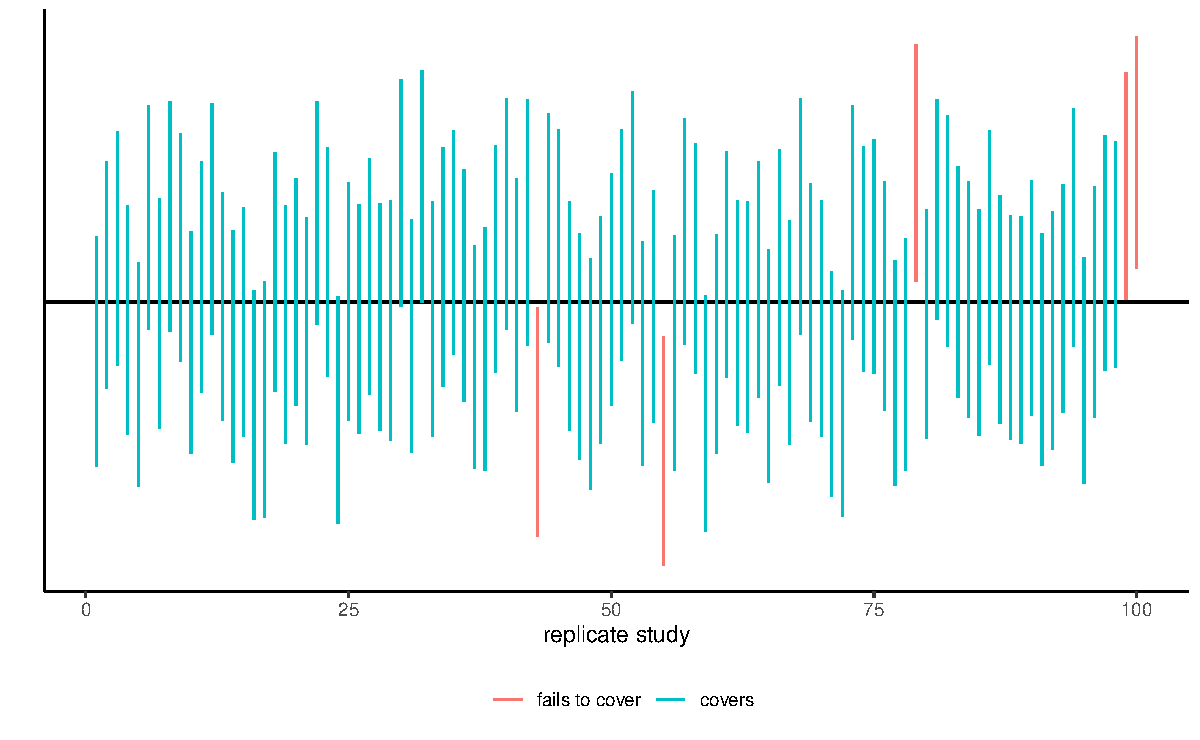
\includegraphics[width=0.85\textwidth,height=\textheight]{inference_files/figure-pdf/intconf-1.pdf}

}

\caption{95\% confidence intervals for the mean of a standard normal
population for 100 random samples. On average, 5\% of these intervals
fail to include the true mean value of zero (in red).}

\end{figure}%

If we are only interested in the binary decision rule reject/fail to
reject \(\mathscr{H}_0,\) the confidence interval is equivalent to a
\emph{p}-value since it leads to the same conclusion. Whereas the
\(1-\alpha\) confidence interval gives the set of all values for which
the test statistic doesn't provide enough evidence to reject
\(\mathscr{H}_0\) at level \(\alpha,\) the \emph{p}-value gives the
probability under the null of obtaning a result more extreme than the
postulated value and so is more precise for this particular value. If
the \emph{p}-value is smaller than \(\alpha,\) our null value \(\theta\)
will be outside of the confidence interval and vice-versa.

\section{Conclusion}\label{conclusion}

The \emph{p}-value allows us to make a decision about the null
hypothesis. If \(\mathscr{H}_0\) is true, the \emph{p}-value follows a
uniform distribution. \href{https://xkcd.com/1478/}{Thus, if the
\emph{p}-value is small}, this means observing an outcome more extreme
than \(T=t\) is unlikely, and so we're inclined to think that
\(\mathscr{H}_0\) is not true. There's always some underlying risk that
we're making a mistake when we make a decision. In statistic, there are
\href{https://xkcd.com/2303/}{two type of errors}:

\begin{itemize}
\tightlist
\item
  type I error: we reject \(\mathscr{H}_0\) when \(\mathscr{H}_0\) is
  true,
\item
  type II error: we fail to reject \(\mathscr{H}_0\) when
  \(\mathscr{H}_0\) is false.
\end{itemize}

These hypothesis are not judged equally: we seek to avoid error of type
I (judicial errors, corresponding to condamning an innocent). To prevent
this, we fix a the level of the test, \(\alpha,\) which captures our
tolerance to the risk of commiting a type I error: the higher the level
of the test \(\alpha,\) the more often we will reject the null
hypothesis when the latter is true. The value of \(\alpha \in (0, 1)\)
is the probability of rejecting \(\mathscr{H}_0\) when \(\mathscr{H}_0\)
is in fact true, \begin{align*}
\alpha = \Pr{}_0\left(\text{ reject } \mathscr{H}_0\right).
\end{align*} where the subscript \(\Pr{}_0\) indicates the probability
under the null model. The level \(\alpha\) is fixed beforehand,
typically \(1\)\%, \(5\)\% or \(10\)\%. Keep in mind that the
probability of type I error is \(\alpha\) only if the null model for
\(\mathscr{H}_0\) is correct (sic) and correspond to the data generating
mechanism.

The focus on type I error is best understood by thinking about medical
trial: you need to prove a new cure is better than existing alternatives
drugs or placebo, to avoid extra costs or harming patients (think of
Didier Raoult and his unsubstantiated claims that hydrochloroquine, an
antipaludean drug, should be recommended treatment against Covid19).

\begin{longtable}[]{@{}lcc@{}}
\toprule\noalign{}
\textbf{Decision} \textbackslash{} \textbf{true model} &
\(\mathscr{H}_0\) & \(\mathscr{H}_a\) \\
\midrule\noalign{}
\endhead
\bottomrule\noalign{}
\endlastfoot
fail to reject \(\mathscr{H}_0\) & \(\checkmark\) & type II error \\
reject \(\mathscr{H}_0\) & type I error & \(\checkmark\) \\
\end{longtable}

To make a decision, we compare our \emph{p}-value \(P\) with the level
of the test \(\alpha\):

\begin{itemize}
\tightlist
\item
  if \(P < \alpha,\) we reject \(\mathscr{H}_0\);
\item
  if \(P \geq \alpha,\) we fail to reject \(\mathscr{H}_0.\)
\end{itemize}

Do not mix up level of the test (probability fixed beforehand by the
researcher) and the \emph{p}-value. If you do a test at level 5\%, the
probability of type I error is by definition \(\alpha\) and does not
depend on the \emph{p}-value. The latter is conditional probability of
observing a more extreme likelihood given the null distribution
\(\mathscr{H}_0\) is true.

\begin{tcolorbox}[enhanced jigsaw, colframe=quarto-callout-caution-color-frame, title=\textcolor{quarto-callout-caution-color}{\faFire}\hspace{0.5em}{Caution}, opacityback=0, leftrule=.75mm, colbacktitle=quarto-callout-caution-color!10!white, breakable, bottomrule=.15mm, toprule=.15mm, toptitle=1mm, opacitybacktitle=0.6, left=2mm, bottomtitle=1mm, colback=white, arc=.35mm, coltitle=black, titlerule=0mm, rightrule=.15mm]

The \href{https://doi.org/10.1080/00031305.2016.1154108}{American
Statistical Association (ASA) published a list of principles} guiding
(mis)interpretation of \emph{p}-values, some of which are reproduced
below:

\begin{quote}
\begin{enumerate}
\def\labelenumi{(\arabic{enumi})}
\setcounter{enumi}{1}
\tightlist
\item
  \emph{P}-values do not measure the probability that the studied
  hypothesis is true.
\end{enumerate}
\end{quote}

\begin{quote}
\begin{enumerate}
\def\labelenumi{(\arabic{enumi})}
\setcounter{enumi}{2}
\tightlist
\item
  Scientific conclusions and business or policy decisions should not be
  based only on whether a \emph{p}-value passes a specific threshold.
\end{enumerate}
\end{quote}

\begin{quote}
\begin{enumerate}
\def\labelenumi{(\arabic{enumi})}
\setcounter{enumi}{3}
\tightlist
\item
  \emph{P}-values and related analyses should not be reported
  selectively.
\end{enumerate}
\end{quote}

\begin{quote}
\begin{enumerate}
\def\labelenumi{(\arabic{enumi})}
\setcounter{enumi}{4}
\tightlist
\item
  \emph{p}-value, or statistical significance, does not measure the size
  of an effect or the importance of a result.
\end{enumerate}
\end{quote}

\end{tcolorbox}

\section{Power}\label{power}

There are two sides to an hypothesis test: either we want to show it is
not unreasonable to assume the null hypothesis, or else we want to show
beyond reasonable doubt that a difference or effect is significative:
for example, one could wish to demonstrate that a new website design
(alternative hypothesis) leads to a significant increase in sales
relative to the status quo. Our ability to detect these improvements and
make discoveries depends on the power of the test: the larger the power,
the greater our ability to reject \(\mathscr{H}_0\) when the latter is
false.

Failing to reject \(\mathscr{H}_0\) when \(\mathscr{H}_a\) is true
corresponds to the definition of type II error, the probability of which
is \(1-\text{power},\) say. The \textbf{power of a test} is the
probability of rejecting \(\mathscr{H}_0\) when \(\mathscr{H}_0\) is
false, i.e., \begin{align*}
\Pr{\!}_a(\text{reject } \mathscr{H}_0),
\end{align*} i.e., the probability under the alternative model of
falling in the rejection region. Depending on the alternative models, it
is more or less easy to detect that the null hypothesis is false and
reject in favor of an alternative.

\begin{figure}[ht!]

\centering{

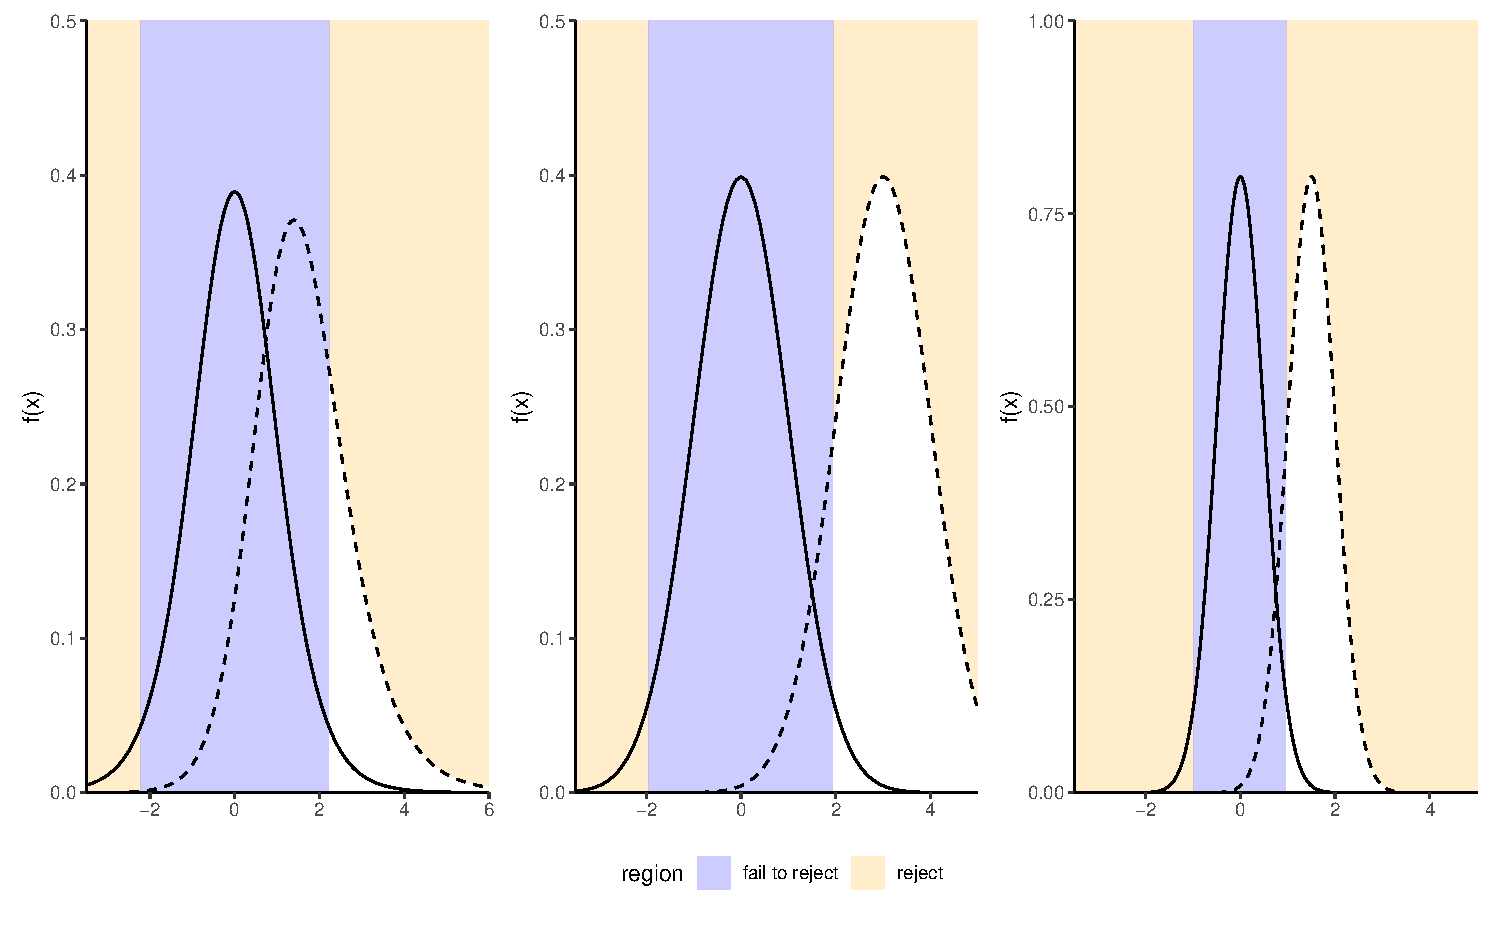
\includegraphics[width=1\textwidth,height=\textheight]{inference_files/figure-pdf/fig-power-1.pdf}

}

\caption{\label{fig-power}Comparison between null distribution (full
curve) and a specific alternative for a \emph{t}-test (dashed line). The
power corresponds to the area under the curve of the density of the
alternative distribution which is in the rejection area (in white). The
middle panel shows an increase in power due to an increase in the mean
difference, whereas the right panel shows the change due to a decrease
in variability of increase in the sample size.}

\end{figure}%

We want a test to have high power, i.e., that the power should be as
close to 1 as possible. Minimally, the power of the test should be
\(\alpha\) because we reject the null hypothesis \(\alpha\) fraction of
the time even when \(\mathscr{H}_0\) is true. Power depends on many
criteria, notably

\begin{itemize}
\tightlist
\item
  the effect size: the bigger the difference between the postulated
  value for \(\theta_0\) under \(\mathscr{H}_0\) and the observed
  behavior, the easier it is to detect it, as in the middle panel of
  Figure~\ref{fig-power};
\item
  variability: the less noisy your data, the easier it is to detect
  differences between the curves (big differences are easier to spot, as
  the right panel of Figure~\ref{fig-power} shows);
\item
  the sample size: the more observation, the higher our ability to
  detect significative differences because the standard error decreases
  with sample size \(n\) at a rate (typically) of \(n^{-1/2}.\) The null
  distribution also becomes more concentrated as the sample size
  increase.
\item
  the choice of test statistic: for example, rank-based statistics
  discard information about the actual values and care only about
  relative ranking. Resulting tests are less powerful, but are typically
  more robust to model misspecification and outliers. The statistics we
  will choose are standard and amongst the most powerful: as such, we
  won't dwell on this factor.
\end{itemize}

To calculate the power of a test, we need to single out a specific
alternative hypothesis. In very special case, analytic derivations are
possible but typically we compute the power of a test through Monte
Carlo methods. For a given alternative, we simulate repeatedly samples
from the model, compute the test statistic on these new samples and the
associated \emph{p}-values based on the postulated null hypothesis. We
can then calculate the proportion of tests that lead to a rejection of
the null hypothesis at level \(\alpha,\) namely the percentage of
\emph{p}-values smaller than \(\alpha.\)

\section{Examples}\label{examples}

\begin{example}[Gender inequality and permutation
tests]\protect\hypertarget{exm-rosenjerdee74}{}\label{exm-rosenjerdee74}

We consider data from Rosen and Jerdee
(\citeproc{ref-Rosen:1974}{1974}), who look at sex role stereotypes and
their impacts on promotion and opportunities for women candidates. The
experiment took place in 1972 and the experimental units, which
consisted of 95 male bank supervisors, were submitted to various
memorandums and asked to provide ratings or decisions based on the
information provided.

We are interested in Experiment 1 related to promotion of employees:
managers were requested to decide on whether or not to promote an
employee to become branch manager based on recommendations and ratings
on potential for customer and employee relations.

The authors intervention focused on the description of the nature
(complexity) of the manager's job (either simple or complex) and the sex
of the candidate (male or female): all files were otherwise similar.

We consider for simplicity only sex as a factor and aggregate over job
for the \(n=93\) replies. Table~\ref{tbl-rosen-table1} shows the counts
for each possibility.

\begin{longtable}[t]{lrr}

\caption{\label{tbl-rosen-table1}Promotion recommandation to branch
manager based on sex of the applicant.}

\tabularnewline

\toprule
 & male & female\\
\midrule
promote & 32 & 19\\
hold file & 12 & 30\\
\bottomrule

\end{longtable}

The null hypothesis of interest here that sex has no impact, so the
probability of promotion is the same for men and women. Let
\(p_{\text{m}}\) and \(p_{\text{w}}\) denote these respective
probabilities; we can thus write mathematically the null hypothesis as
\(\mathscr{H}_0: p_{\text{m}} = p_{\text{w}}\) against the alternative
\(\mathscr{H}_a: p_{\text{m}} \neq p_{\text{w}}.\)

The test statistic typically employed for contingency tables is a
chi-square test\footnote{If you have taken advanced modelling courses,
  this is a score test obtained by fitting a Poisson regression with
  \texttt{sex} and \texttt{action} as covariates; the null hypothesis
  corresponding to lack of interaction term between the two.}, which
compares the overall proportions of promoted to that in for each
subgroup. The sample proportion for male is 32/42 = \textasciitilde76\%,
compared to 19/49 or \textasciitilde49\% for female. While it seems that
this difference of 16\% is large, it could be spurious: the standard
error for the sample proportions is roughly 3.2\% for male and 3.4\% for
female.

If there was no discrimination based on sex, we would expect the
proportion of people promoted to be the same overall; this is 51/93
=0.55 for the pooled sample. We could simply do a test for the mean
difference, but rely instead on the Pearson contingency \(X^2_p\) (aka
chi-square) test, which compares the expected counts (based on equal
promotion rates) to the observed counts, suitably standardized. If the
discrepancy is large between expected and observed, than this casts
doubt on the validity of the null hypothesis.

If the counts of each cell are large, the null distribution of the
chi-square test is well approximated by a \(\chi^2\) distribution. The
output of the test includes the value of the statistic, \(10.79,\) the
degrees of freedom of the \(\chi^2\) approximation and the
\emph{p}-value, which gives the probability that a random draw from a
\(\chi^2_1\) distribution is larger than the observed test statistic
\textbf{assuming the null hypothesis is true}. The \emph{p}-value is
very small, \(0.001,\) which means such a result is quite unlikely to
happen by chance if there was no sex-discrimination.

Another alternative to obtain a benchmark to assess the outlyingness of
the observed odds ratio is to use simulations: permutation tests are
well \href{https://www.jwilber.me/permutationtest/}{illustrated by Jared
Wilber}. Consider a database containing the raw data with 93 rows, one
for each manager, with for each an indicator of \texttt{action} and the
\texttt{sex} of the hypothetical employee presented in the task.

\begin{longtable}[t]{ll}

\caption{\label{tbl-dat-long-test-rosen-print}First five rows of the
database in long format for experiment 1 of Rosen and Jerdee.}

\tabularnewline

\toprule
action & sex\\
\midrule
promote & male\\
hold file & female\\
promote & male\\
hold file & female\\
hold file & male\\
\bottomrule

\end{longtable}

Under the null hypothesis, sex has no incidence on the action of the
manager. This means we could get an idea of the ``what-if'' world by
shuffling the sex labels repeatedly. Thus, we could obtain a benchmark
by repeating the following steps multiple times:

\begin{enumerate}
\def\labelenumi{\arabic{enumi}.}
\tightlist
\item
  permute the labels for \texttt{sex},
\item
  recreate a contingency table by aggregating counts,
\item
  calculate a test statistic for the simulated table.
\end{enumerate}

As test statistic, we use odds ratio: the odds of an event is the ratio
of the number of success over failure: in our example, this would be the
number of promoted over held files. The odds of promotion for male is
\(32/12,\) whereas that of female is \(19/30.\) The odds ratio for male
versus female is thus \(\mathsf{OR}=(32/12) / (19/30)= 4.21.\) Under the
null hypothesis, \(\mathscr{H}_0: \mathsf{OR}= 1\) (same probability of
being promoted) (why?)

\begin{figure}[ht!]

\centering{

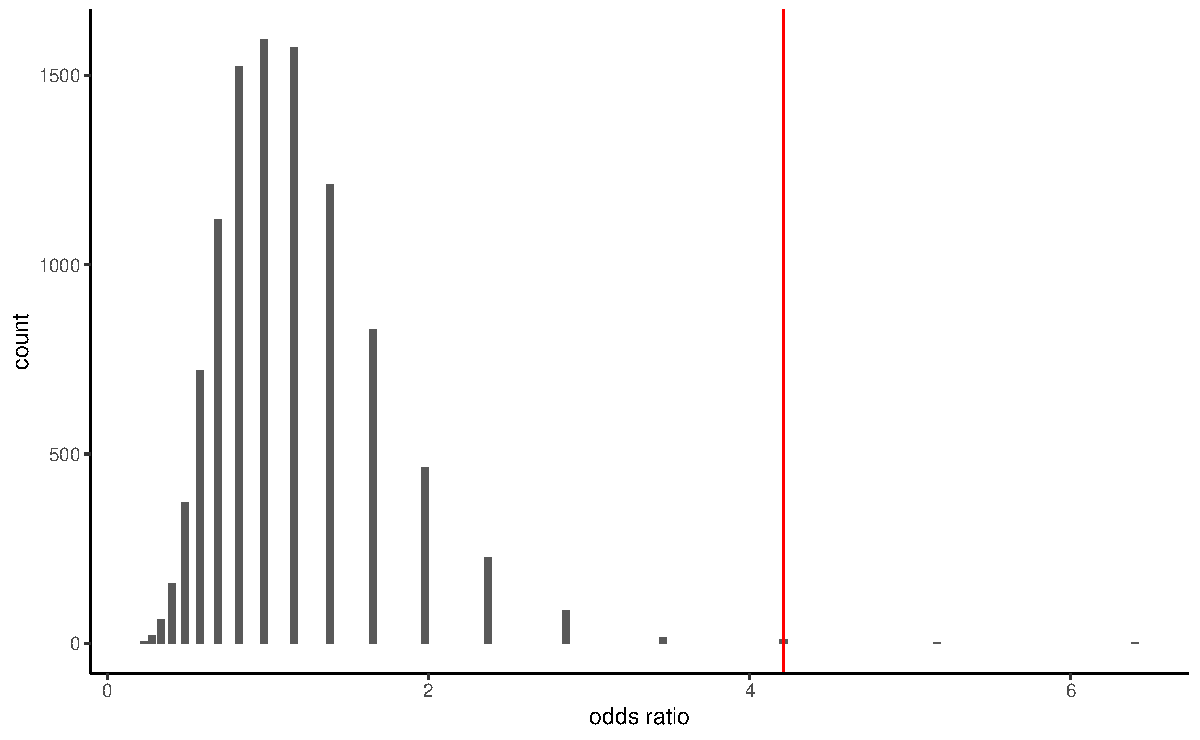
\includegraphics[width=0.85\textwidth,height=\textheight]{inference_files/figure-pdf/fig-infer-odds-ratio-permutation-1.pdf}

}

\caption{\label{fig-infer-odds-ratio-permutation}Histogram of the
simulated null distribution of the odds ratio statistic obtained using a
permutation test; the vertical red line indicates the sample odds
ratio.}

\end{figure}%

The histogram in Figure~\ref{fig-infer-odds-ratio-permutation} shows the
distribution of the odds ratio based on 10 000 permutations.
Reassuringly, we again get roughly the same approximate \emph{p}-value,
here 0.002.\footnote{The \emph{p}-value obtained for the permutation
  test would change from one run to the next since it's input is random.
  However, the precision of the proportion statistic is sufficient for
  decision making purposes.}

The article concluded (in light of the above and further experiments)

\begin{quote}
Results confirmed the hypothesis that male administrators tend to
discriminate against female employees in personnel decisions involving
promotion, development, and supervision.
\end{quote}

\textbf{Recap}

\begin{itemize}
\tightlist
\item
  Model parameters: probability of promotion for men and women,
  respectively \(p_{\text{m}}\) and \(p_{\text{w}}.\)
\item
  Hypotheses: no discrimination based on gender, meaning equal
  probability of promotion (null hypothesis
  \(\mathscr{H}_0: p_{\text{m}}=p_{\text{w}},\) versus alternative
  hypothesis \(\mathscr{H}_a: p_{\text{m}}\neq p_{\text{w}}\)).
\item
  Test statistic: (1) chi-square test for contingency tables and (2)
  odds ratio.
\item
  \(p\)-value: (1) \(.0010\) and (2) \(.0024\) based on permutation
  test.
\item
  Conclusion: reject null hypothesis, as there is evidence of a
  gender-discrimination with different probability of promotion for men
  and women.
\end{itemize}

Following the APA guidelines, the \(\chi^2\) statistic would be reported
as \(\chi^2(1, n = 93) = 10.79\), \(p = .001\) along with counts and
sample proportions.

\end{example}

\begin{example}[``The Surprise of Reaching
Out'']\protect\hypertarget{exm-LiuRimMinMin2023E1}{}\label{exm-LiuRimMinMin2023E1}

Liu et al. (\citeproc{ref-Liu.Rim.Min.Min:2023}{2023}) studies social
interactions and the impact of surprise on people reaching out if this
contact is unexpected. Experiment 1 focuses on questionnaires where the
experimental condition is the perceived appreciation of reaching out to
someone (vs being reached to). The study used a questionnaire
administered to 200 American adults recruited on the Prolific Academic
platform. The response index consists of the average of four questions
measured on a Likert scale ranging from 1 to 7, with higher values
indicating higher appreciation.

We can begin by inspecting summary statistics for the sociodemographic
variables (gender and age) to assess whether the sample is
representative of the general population as a whole. The proportion of
\texttt{other} (including non-binary people) is much higher than that of
the general census, and the population skews quite young according to
Table~\ref{tbl-LRMMS1-summarystat-a}.

\begin{longtable}[t]{lrrrr}

\caption{\label{tbl-LRMMS1-summarystat-a}Summary statistics of the age
of participants, and counts per gender}

\tabularnewline

\toprule
gender & min & max & mean & n\\
\midrule
male & 18 & 78 & 32.0 & 105\\
female & 19 & 68 & 36.5 & 92\\
other & 24 & 30 & 27.7 & 3\\
\bottomrule

\end{longtable}

\begin{longtable}[t]{lrrr}

\caption{\label{tbl-LRMMS1-summarystat-b}Mean ratings, standard
deviation and number of participants per experimental condition.}

\tabularnewline

\toprule
role & mean & sd & n\\
\midrule
initiator & 5.50 & 1.28 & 103\\
responder & 5.87 & 1.27 & 97\\
\bottomrule

\end{longtable}

Since there are only two groups, initiator and responder, we are dealing
with a pairwise comparison. The logical test one could use is a two
sample \emph{t}-test, or a variant thereof. Using Welch two sample
\(t\)-test statistic, both group average and standard deviation are
estimated using the data provided.

The software returns \(t(197.52) = -2.05\), \(p = .041\), which leads to
the rejection of the null hypothesis of no difference in appreciation
depending on the role of the individual (initiator or responder). The
estimated mean difference is \(\Delta M = -0.37\), 95\% CI
\([-0.73, -0.01]\); since \(0\) is not included in the confidence
interval, we also reject the null hypothesis at level 5\%. The estimate
suggests that initiators underestimate the appreciation of reaching
out.\footnote{Assuming that the variance of each subgroup were equal, we
  could have used a two-sample \(t\)-test instead. The difference in the
  conclusion is immaterial, with a nearly equal \emph{p}-value.}

\textbf{Recap}

\begin{itemize}
\tightlist
\item
  Model parameters: average expected appreciation score
  \(\mu_{\mathrm{i}}\) and \(\mu_{\mathrm{r}}\) of initiators and
  responder, respectively
\item
  Hypothesis: expected appreciation score is the same for initiator and
  responders, \(\mathscr{H}_0: \mu_{\mathrm{i}}=\mu_{\mathrm{r}}\)
  against alternative
  \(\mathscr{H}_a: \mu_{\mathrm{i}} \neq \mu_{\mathrm{r}}\) that they
  are different.
\item
  Test statistic: Welch two sample \(t\)-test
\item
  \(p\)-value: 0.041
\item
  Conclusion: reject the null hypothesis, average appreciation score
  differs depending on the role
\end{itemize}

\end{example}

\begin{example}[Virtual communication curbs creative idea
generation]\protect\hypertarget{exm-BrucksLevav22}{}\label{exm-BrucksLevav22}

A Nature study performed an experiment to see how virtual communications
teamwork by comparing the output both in terms of ideas generated during
a brainstorming session by pairs and of the quality of ideas, as
measured by external referees. The sample consisted of 301 pairs of
participants who interacted via either videoconference or face-to-face.

The authors compared the number of creative ideas, a subset of the ideas
generated with creativity score above average. The mean number of the
number of creative ideas for face-to-face \(7.92\) ideas (sd \(3.40\))
relative to videoconferencing \(6.73\) ideas (sd \(3.27\)).

Brucks and Levav (\citeproc{ref-Brucks.Levav:2022}{2022}) used a
negative binomial regression model: in their model, the expected number
creative ideas generated is \begin{align*}
\mathsf{E}(\texttt{ncreative}) = \exp(\beta_0 + \beta_1 \texttt{video})
\end{align*} where \(\texttt{video}=0\) if the pair are in the same room
and \(\texttt{video}=1\) if they interact instead via videoconferencing.

The mean number of ideas for videoconferencing is thus \(\exp(\beta_1)\)
times that of the face-to-face: the estimate of the multiplicative
factor is \(\exp(\beta_1)\) is \(0.85\) 95\% CI \([0.77, 0.94]\).

No difference between experimental conditions translates into the null
hypothesis as \(\mathscr{H}_0: \beta_1=0\) vs
\(\mathscr{H}_0: \beta_1 \neq 0\) or equivalently
\(\mathscr{H}_0: \exp(\beta_1)=1.\) The likelihood ratio test comparing
the regression model with and without \(\texttt{video}\) the statistic
is \(R=9.89\) (\(p\)-value based on \(\chi^2_1\) of \(.002\)). We
conclude the average number of ideas is different, with summary
statistics suggesting that virtual pairs generate fewer ideas.

If we had resorted to a two sample \(t\)-test, we would have found a
mean difference in the number of creative idea of \(\Delta M = 1.19\),
95\% CI \([0.43, 1.95]\), \(t(299) = 3.09\), \(p = .002\).

Both tests come with slightly different sets of assumptions, but yield
similar conclusions: there is evidence of a smaller number of creative
ideas when people interact via videoconferencing.

\end{example}

\begin{example}[Price of Spanish high speed train
tickets]\protect\hypertarget{exm-price-trains-tests}{}\label{exm-price-trains-tests}

The Spanish national railway company,
\href{https://www.renfe.com/}{Renfe}, manages regional and high speed
train tickets all over Spain and The Gurus
\href{https://www.kaggle.com/thegurusteam/spanish-high-speed-rail-system-ticket-pricing}{harvested}
the price of tickets sold by Renfe. We are interested in trips between
Madrid and Barcelona and, for now, ask the question: are tickets more
expensive one way or another? To answer this, we consider a sample of
8059 AVE tickets sold at Promo rate. Our test statistic will again be
the mean difference between the price (in euros) for a train ticket for
Madrid--Barcelona (\(\mu_1\)) and the price for Barcelona--Madrid
(\(\mu_2\)), i.e., \(\mu_1-\mu_2.\) The null hypothesis is that there
are no difference in price, so \(\mathscr{H}_0: \mu_1-\mu_2=0.\)

We use Welch's \(t\) test statistic for two samples: the sample mean of
the price of Barcelona-Madrid tickets is 82.15 euros, that of
Madrid-Barcelona tickets is 82.54 euros and the Welch statistic is worth
-1.15. If we use a normal approximation, the \emph{p}-value is 0.25.

Rather than use the asymptotic distribution, whose validity stems from
the central limit theorem, we could consider another approximation under
the less restrictive assumption that the data are exchangeable: under
the null hypothesis, there is no difference between the two destinations
and so the label for destination (a binary indicator) is arbitrary. The
reasoning underlying
\href{https://www.jwilber.me/permutationtest/}{permutation tests} is as
follows: to create a benchmark, we will consider observations with the
same number in each group, but permuting the labels. We then compute the
test statistic on each of these datasets. If there are only a handful in
each group (fewer than 10), we could list all possible permutations of
the data, but otherwise we can repeat this procedure many times, say
9999, to get a good approximation. This gives an approximate
distribution from which we can extract the \emph{p}-value by computing
the rank of our statistic relative to the others.

\begin{figure}[ht!]

\centering{

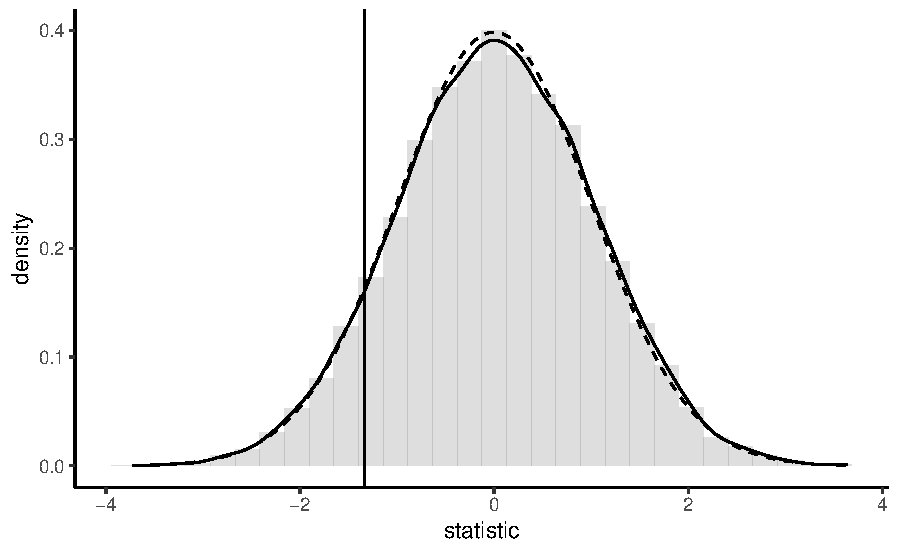
\includegraphics[width=0.85\textwidth,height=\textheight]{inference_files/figure-pdf/fig-renfepermut-1.pdf}

}

\caption{\label{fig-renfepermut}Permutation-based approximation to the
null distribution of Welch two-sample t-test statistic (histogram and
black curve) with standard normal approximation (dashed curve) for the
price of AVE tickets at promotional rate between Madrid and Barcelona.
The value of the test statistic calculated using the original sample is
represented by a vertical line.}

\end{figure}%

The so-called bootstrap approximation to the \emph{p}-value of the
permutation test, \(0.186,\) is the proportion of statistics that are
more extreme than the one based on the original sample. It is nearly
identical to that obtained from the Satterthwaite approximation,
\(0.249\) (the Student-\(t\) distribution is numerically equivalent to a
standard normal with that many degrees of freedom), as shown in
Figure~\ref{fig-renfepermut}. Even if our sample is very large
(\(n=8059\) observations), the difference is not statistically
significative. With a bigger sample (the database has more than 2
million tickets), we could estimate more precisely the average
difference, up to 1/100 of an euro: the price difference would
eventually become statistically significative, but this says nothing
about practical difference: \(0.28\) euros relative to an Promo ticket
priced on average \(82.56\) euros is a negligible amount.

\end{example}

\bookmarksetup{startatroot}

\chapter*{Bibliography}\label{bibliography}
\addcontentsline{toc}{chapter}{Bibliography}

\markboth{Bibliography}{Bibliography}

\phantomsection\label{refs}
\begin{CSLReferences}{1}{0}
\bibitem[\citeproctext]{ref-Brodeur:2021}
Brodeur, Mathieu, Perrine Ruer, Pierre-Majorique Léger, and Sylvain
Sénécal. 2021. {``Smartwatches Are More Distracting Than Mobile Phones
While Driving: Results from an Experimental Study.''} \emph{Accident
Analysis \& Prevention} 149: 105846.
\url{https://doi.org/10.1016/j.aap.2020.105846}.

\bibitem[\citeproctext]{ref-Brucks.Levav:2022}
Brucks, Melanie S., and Jonathan Levav. 2022. {``Virtual Communication
Curbs Creative Idea Generation.''} \emph{Nature} 605 (7908): 108--12.
\url{https://doi.org/10.1038/s41586-022-04643-y}.

\bibitem[\citeproctext]{ref-Duke.Amir:2023}
Duke, Kristen E., and On Amir. 2023. {``The Importance of Selling
Formats: When Integrating Purchase and Quantity Decisions Increases
Sales.''} \emph{Marketing Science} 42 (1): 87--109.
\url{https://doi.org/10.1287/mksc.2022.1364}.

\bibitem[\citeproctext]{ref-Student:1908}
Gosset, William Sealy. 1908. {``The Probable Error of a Mean.''}
\emph{Biometrika} 6 (1): 1--25.
\url{https://doi.org/10.1093/biomet/6.1.1}.

\bibitem[\citeproctext]{ref-Lee.Choi:2019}
Lee, Kiljae, and Jungsil Choi. 2019. {``Image-Text Inconsistency Effect
on Product Evaluation in Online Retailing.''} \emph{Journal of Retailing
and Consumer Services} 49: 279--88.
\url{https://doi.org/10.1016/j.jretconser.2019.03.015}.

\bibitem[\citeproctext]{ref-Liu.Rim.Min.Min:2023}
Liu, Peggy J., SoYon Rim, Lauren Min, and Kate E. Min. 2023. {``The
Surprise of Reaching Out: Appreciated More Than We Think.''}
\emph{Journal of Personality and Social Psychology} 124 (4): 754--71.
\url{https://doi.org/10.1037/pspi0000402}.

\bibitem[\citeproctext]{ref-Moon.VanEpps:2023}
Moon, Alice, and Eric M VanEpps. 2023. {``Giving Suggestions: Using
Quantity Requests to Increase Donations.''} \emph{Journal of Consumer
Research} 50 (1): 190--210. \url{https://doi.org/10.1093/jcr/ucac047}.

\bibitem[\citeproctext]{ref-Rosen:1974}
Rosen, B., and T. H. Jerdee. 1974. {``Influence of Sex Role Stereotypes
on Personnel Decisions.''} \emph{Journal of Applied Psychology} 59:
9--14.

\bibitem[\citeproctext]{ref-Sokolova:2023}
Sokolova, Tatiana, Aradhna Krishna, and Tim Döring. 2023. {``Paper Meets
Plastic: The Perceived Environmental Friendliness of Product
Packaging.''} \emph{Journal of Consumer Research} 50 (3): 468--91.
\url{https://doi.org/10.1093/jcr/ucad008}.

\end{CSLReferences}


\backmatter


\end{document}
